\documentclass[12pt,twoside]{article}
\title{M374M Notes}
\author{Hershal Bhave (hb6279)}
\date{Updated \today \\ \normalsize{Revision \input{revision}}}

\usepackage{homework-macros}
\usetikzlibrary{plotmarks}
\tikzexternalize

\begin{document}
\maketitle
\tableofcontents

\section{Dimensional Analysis}
\subsection{Example}
Let $q = \alpha p^2$, where $[\alpha] = \frac{L}{T^2}$, $[p] = T$. Find $[q]$,
$\left[\frac{dq}{dp}\right]$.

\subsection{Definition}
$q$ is \emph{dimensionless} if $[q] = 1$. Angles are dimensionless, for example.

\subsection{Examples}
\subsubsection{}
Let $y = f(x)$, where $[y] = [x]$. Then $\frac{dy}{dx}$ is dimensionless.

\subsubsection{}
By definition, pure numbers are dimensionless

\begin{equation}
  \begin{aligned}
    g &= 10 \text{m}/\text{s}^2 \\
    g + g &= 2g = 20 \text{m}/\text{s}^2 \\
    g \cdot g \cdot g & = g^3 = 1000 \text{m}^3/\text{s}^6
  \end{aligned}
\end{equation}

\subsection{Remark}
Some functions make dimensional sense only if inputs are dimensionless.

\begin{equation}
  \begin{aligned}
    e^q &= 1 + q + \frac{q^2}{2!} + \frac{q^3}{3!} + \cdots \\
    [q] &= 1 \implies [e^q] = 1 \\
    [q] &= L \implies [e^q] = ?
  \end{aligned}
\end{equation}

\subsection{Definition}
An equation in ``standard form'' $F(q, p, \ldots) = 0$ is called unit-free if
each term has the same dimenison.

\subsection{Example}
Galileo's Law.

\begin{equation}
  \begin{aligned}
    x &= \frac{gt^2}{2} \\
    x - \frac{gt^2}{2} &= 0 \\
    F(x,t,g) &= 0
  \end{aligned}
\end{equation}

Where $[x] = L$, $[\frac{gt^2}{2}] = [gt^2] = L$.
$\therefore F(x,t,g)=0$ is unit-free.

\subsection{Remarks}
\begin{enumerate}
\item All equations we consider are unit-free
\item Differentiation, integration preserves unit-free propery of an equation
\end{enumerate}

\begin{equation}
  \begin{aligned}
    \frac{d^2x}{dt^2} &= g \text{unit-free} \\
    \frac{dx}{dt} &= gt + v_0 \\
    x &= \frac{1}{2}gt^2 + v_0 t + x_0 \\
  \end{aligned}
  %% $\therefore$ unit-free ODE $\implies$ unit-free solution.
\end{equation}

\subsection{Definition}
Let $Q = {q_1, \ldots, q_m}$ be a set of quantities involving a set $D =
{D_1,\ldots,D_n}$ of dimensions so that

\begin{equation}
  \begin{aligned}
    [q_1] &= D_1^{a_{11}} D_2^{a_{21}}\cdots D_n^{a_{n1}} \\
    \vdots & \\
    [q_2] &= D_1^{a_{21}} D_2^{a_{22}}\cdots D_n^{a_{n2}} \\
  \end{aligned}
\end{equation}
for some exponents $a_{11}, \ldots, a_{nm}$.

By the dimension matrix for $Q$, $D$, we mean
\begin{equation}
  A =
  \begin{pmatrix}
    a11 & a12 & \cdots & a1m \\
    a21 & a22 & \cdots & a2m \\
    \vdots & & & \\
    an1 & an2 & \cdots & anm \\
  \end{pmatrix}
  \in \mathbb{R}^{n\times m}
\end{equation}

\subsection{Example}
$m = 3 | Q = {x, t, g}$, $n = 2 | D = {L, T}$.
\begin{equation}
  \begin{aligned}
    [x] &= L^1 T^0 \\
    [t] &= L^0 T^1 \\
    [g] &= L^1 T^{-2}
  \end{aligned}
\end{equation}

\begin{equation}
  A =
  \begin{pmatrix}
    1 & 0 & 1 \\
    0 & 1 & -2 \\
  \end{pmatrix}
  \in \mathbb{R}^{2\times3}
\end{equation}

\subsection{Remarks}
All dimensionless combinations of $q_1,\ldots,q_m$ can be found from the null
vectors of $A$. That is,

$$Z = q_1^{v_1}, q_2^{v_2}, \ldots, q_n^{v_n}$$ where $v_1, \ldots, v_m$
arbitrary. Then
\begin{equation}
  \begin{aligned}
    [Z] &= 1 \rightleftarrows Av=0, \\
    v &= \begin{pmatrix} v_1 \\ \vdots \\ v_m \end{pmatrix}
  \end{aligned}
\end{equation}

\subsection{Example}
Find all dimensionless combinations of $x, t, g$.

\begin{equation}
  \begin{aligned}
    Z &= x^{v_1}t^{v_2}g^{v_3} \\
    [Z] &= {[x]}^{v_1}{[t]}^{v_2}{[g]}^{v_3} \\
    &= L^{v_1}T^{v_2}{(LT^{-2})}^{v_3} \\
    &= L^{v_1+v_3} T^{v_2-2v_3} \\
    \implies [Z] = 1 & \rightleftarrows  v_1+v_3=0, v_2-2v^3=0
  \end{aligned}
\end{equation}

\begin{equation}
  \begin{aligned}
    \begin{pmatrix}
      1 & 0 & 1 \\
      0 & 1 & -2
    \end{pmatrix}
    \begin{pmatrix}
      v_1 \\ v_2 \\ v_3 \\
    \end{pmatrix}
    &=
    \begin{pmatrix}
      0 \\ 0
    \end{pmatrix}
    \implies Av &= 0
  \end{aligned}
\end{equation}

\begin{equation}
  v = c
  \begin{pmatrix}
    -1 & 2 & 1
  \end{pmatrix}
\end{equation}
Where $c$ is free.
\begin{equation}
  \begin{aligned}
    c &= 1 \rightarrow v =
    \begin{pmatrix}
      -1 \\ 2 \\ 1
    \end{pmatrix} \rightarrow
    Z = x^{-1} t^2 g^1 = \frac{t^2g}{x} \\
    c &= 2 \rightarrow v=
    \begin{pmatrix}
      -2 \\ 4 \\ 2
    \end{pmatrix} \rightarrow
    Z = \frac{t^4g^1}{x^2}
  \end{aligned}
\end{equation}
The cases where $c=1$ and $c=2$ are the same combination, so we don't have
independent results.

\section{Characteristic Scales}
\subsection{Definition}
Non-zero constants $t_c$, $y_c$ are called characteristic scales for a function
$y=f(t)$ if the following is true:

\begin{enumerate}
\item \begin{itemize}
\item $[t_c] = [t]$
\item $[y_c] = [t]$
\end{itemize}

\item Main features of $y=f(t)$ graph are clearly visible in a $mt_c \times ny_c$
   window for moderate values of $m,n$ ($1 \le m, \; n \le 10$).
\end{enumerate}

\subsection{Examples}
\subsubsection{Example 1}
$y=A\sin(\pi t/b), t \ge 0$, $A$, $b$ constants, $A = 1 \text{ meter}$, $b=1
\text{ second}$. Reference fig. 1.1.

Characteristic scales are $t_c=b, y_c=A$ since $2b \times 2A$ window captures
main features of graph.

Can understand the features of the graph within this window. Reference fig. 1.2.

Windows of significantly different sizes would give poor representations of
functions. Reference fig. 1.3.

\subsubsection{Example 2}
$y = Ae^{-t/b}, t\ge0$ where $[y]=L$, $[t] = T$, $A$, $b$ constants.

Reference fig. 1.4. Characteristic scales are $t_c=b$, $y_c=A$ since window
$10b \times A$ captures main features.

\subsubsection{Example 3}
Fig. 1.5 has two sets of characteristic scales; two window sizes are needed to
represent the features, as shown in figs. 1.6 and 1.7.

\subsection{Procedure}
Given some (potentially indirect) definition of a graph, how do we indentify the
scales?

If $y=f(t)$ is defined by an equation involving constants $g_1, \ldots, g_m$,
then characteristic scales $t_c$, $y_c$ can be found by solving:

\begin{equation}
  \begin{aligned}
    t_c &= g_1^{\alpha_1}, \ldots, g_m^{\alpha_m} \\
    y_c &= g_1^{\beta_1}, \ldots, g_m^{\beta_m}
  \end{aligned}
\end{equation}

for $\alpha_1, \ldots, \alpha_m$ and $\beta_1, \ldots, \beta_m$.

\subsection{Examples}
\subsubsection{Example 1}

Find characteristic scales $t_c$, $y_c$ for $y=f(t)$ defined by

\begin{equation} \text{(IVP)}\quad
  \left\{
  \begin{aligned}
    \frac{dy}{dt} &= \eta y, \quad t\ge0 \\
    y_{(0)} &= \lambda \\
  \end{aligned} \right.
\end{equation}
$[y] = \Eta , [t]=T$. Dimensions of $\eta$, $\lambda$:
\begin{equation}
  \begin{aligned}
    \frac{\Eta}{T} &= [\eta]\Eta \rightarrow [\eta]=\frac{1}{T} \\
    \Eta &= [\lambda]
  \end{aligned}
\end{equation}
Scales for $t$, $y$:
\begin{multicols}{2}
  \begin{equation}
    \begin{aligned}
      t_c &= \eta^{\alpha_1} \lambda^{\alpha_2} \\
      \implies T &= T^{-\alpha_1}\Eta^{\alpha_2} \\
      \implies \alpha_1 &= -1,\quad \alpha_2 = 0 \\
      \implies t_c &= \frac{1}{\eta}\\
    \end{aligned}
  \end{equation}
\\
  \begin{equation}
    \begin{aligned}
      y_c &= \eta^{\beta_1} \lambda^{\beta_2} \\
      \implies \Eta &= T^{-\beta_1}\Eta^{\beta_2} \\
      \implies \beta_1 &= 0,\quad \beta_2 = 1 \\
      \implies y_c &= \lambda
    \end{aligned}
  \end{equation}
\end{multicols}
\subsubsection{Example 2}

Do the same for
\begin{equation}
  \left\{
  \begin{aligned}
    \frac{d^2y}{dt^2} &= \eta \frac{dy}{dt} + \mu y^2,\quad t \ge 0 \\
    y_{(0)} &= \lambda, \quad \frac{dy}{dt}(0) = 0
  \end{aligned} \right.
\end{equation}
Where $[y]=L$, $[t]=T$, $\eta$, $\mu$, $\lambda$ are constants.

Dimensions of $\eta$, $\mu$, $\lambda$:
\begin{equation}
  \begin{aligned}
    [\lambda] &= L \\
    [\eta]\frac{L}{T} &= \frac{L}{T^2} \quad\longrightarrow\quad [\eta] = \frac{1}{T} \\
    [\mu]L^2 &= \frac{L}{T^2} \quad\longrightarrow\quad [\mu] = \frac{1}{LT^2} \\
  \end{aligned}
\end{equation}

Scale for $t$:
\begin{equation}
  \begin{aligned}
    t_c &= \eta^{\alpha_1}\mu^{\alpha_2}\lambda^{\alpha_3} \\
    &= T^{-\alpha_1}{(L^{-1}T^{-2})}^{\alpha_2}L^{\alpha_3} \\
    \implies L^0T^1 &= L^{-\alpha_2+\alpha_3}T^{\alpha_1-2\alpha_2} \\
  \end{aligned}
\end{equation}

\begin{equation}
  \begin{pmatrix}
    -1 & -2 & 0 \\
    0 & -1 & 1 \\
  \end{pmatrix}
\begin{pmatrix}
  \alpha_1 \\
  \alpha_2 \\
  \alpha_3 \\
\end{pmatrix}
=
\begin{pmatrix}
  1\\0
\end{pmatrix}
\end{equation}

Where $\alpha_3$ is free.

\begin{equation}
  \begin{aligned}
    -\alpha_1-2\alpha_2 &= 1 \rightarrow \alpha_1=-2\alpha_2-1=-2\alpha_3-1\\
    -\alpha_2 + \alpha_3 = 0 \rightarrow \alpha_2&=\alpha_3
  \end{aligned}
\end{equation}

\begin{equation}
  \begin{pmatrix}
    \alpha_1 \\ \alpha_2 \\\alpha_3 \\
  \end{pmatrix}
  =
  \begin{pmatrix}
    -2\alpha_3-1 \\ \alpha_3 \\\alpha_3 \\
  \end{pmatrix}
  = \alpha_3
  \begin{pmatrix}
    -2 \\ 1 \\ 1
  \end{pmatrix}
  +
  \begin{pmatrix}
    -1 \\ 0 \\ 0
  \end{pmatrix}
\end{equation}

Where $\alpha_3$ is free. $\alpha_3=0, \quad \alpha_3\ne0$ gives two scales for
t\_c:

\begin{equation}
  \alpha_3=0, \quad
  \begin{pmatrix}
    -1 \\ 0 \\ 0
  \end{pmatrix}
\end{equation}

\begin{equation}
  \implies t_c = \frac{1}{\eta}.
\end{equation}

And

\begin{equation}
  \alpha_3 = \frac{-1}{2}, \quad
  \begin{pmatrix}
    \alpha_1 \\ \alpha_2 \\ \alpha_3 \\
  \end{pmatrix}
  =
  \begin{pmatrix}
    0 \\ -1/2 \\ -1/2
  \end{pmatrix}
\end{equation}

\begin{equation}
  \implies t_c = \frac{1}{\sqrt{\mu\lambda}}
\end{equation}

Same for $y_c$

\begin{equation}
  \begin{aligned}
    y_c &= \frac{\eta^2}{\mu} \\
    y_c &= \lambda
  \end{aligned}
\end{equation}

\section{Dimensionless Forms}
\subsection{Definition}
Consider an equation involving vars $v_1,\ldots,v_k$. By the dimensionless form
of an equation with respect to scales $v_1^c,\ldots,v_k^c$ we mean the equation
obtained by the substitution $\overline{v_i}=v_i/v_i^c,\quad i=1,\ldots,k$ where
$\overline{v_i}$ is a dimensionless variable.

\subsection{Example}
\begin{equation}
  \left\{
  \begin{aligned}
    \frac{dy}{dt} &= \eta y+r, \quad t\ge0 \\
    y_{(0)} &= \lambda \\
  \end{aligned}
  \right.
\end{equation}

\begin{equation}
  [y] = \Theta,\quad[t]=T,\quad \eta,\lambda,r > 0 \text{ constants}
\end{equation}

Find dimensionless equation with respect to scales
$t_c=\frac{1}{\eta},\quad y_c=\lambda$.

Dimensionless vars
\begin{equation}
  \begin{aligned}
    \bar{y} &= y/y_c = y/\lambda,\quad & \bar{t} &= t/t_c = \eta t \\
    y &= \lambda \bar{y}, \quad & t&=\bar{t}/\eta \\
  \end{aligned}
\end{equation}

Derivitive relation
\begin{equation}
  \begin{aligned}
    \frac{d\bar{y}}{d\bar{t}} &= \frac{d\bar{y}}{dt} \cdot \frac{dt}{d\bar{t}}
  \end{aligned}
\end{equation}

Where $\frac{d\bar{y}}{dt} = \frac{d}{dt}(y/\lambda) = \frac{1}{\lambda}\frac{dy}{dt}$ and
$\frac{dt}{d\bar{t}} = \frac{1}{\eta}$. Thus

\begin{equation}
  \begin{aligned}
    \frac{d\bar{y}}{d\bar{t}} &= \frac{1}{\eta\lambda}\frac{dy}{dt} \\
    \therefore \frac{dy}{dt} &= \eta\lambda\frac{d\bar{y}}{d\bar{t}} \\
  \end{aligned}
\end{equation}

In general, $\frac{dy}{dt} = \frac{y_c}{t_c} \cdot \frac{d\bar{y}}{d\bar{t}}$.
Substituted into equations,

\begin{equation}
  \begin{aligned}
    \frac{dy}{dt} &= \eta y+r, &\quad t&\ge0 \\
    \eta\lambda\frac{d\bar{y}}{d\bar{t}} &= \eta\lambda\bar{y}+r, &\quad \bar{t}/\eta&\ge0 \\
    \frac{d\bar{y}}{d\bar{t}} &= \bar{y}+\frac{r}{\eta\lambda}, &\quad \bar{t}&\ge0 \\
    y &= \lambda, &\quad t&=0 \\
    \lambda\bar{y} &= \lambda, &\quad \bar{t}/\eta &= 0 \\
    \bar{y} &= 1, &\quad\bar{t}&=0. \\
  \end{aligned}
\end{equation}

We end up with dimensionless equations
\begin{equation} \left\{
  \begin{aligned}
    \frac{d\bar{y}}{d\bar{t}} &= \bar{y} + \bar{r}, &\quad \bar{t}&\ge0 \\
    \bar{y} &= 1, &\quad \bar{t} &= 0
  \end{aligned} \right.
\end{equation}

Where $\bar{r} = \frac{r}{\eta\lambda}$ is a dimensionless constant.

\subsection{Remarks}
\begin{enumerate}
\item Different choices of scales lead to different dimensionless equations
  \begin{equation}
    \begin{aligned}
      t_c &= \lambda/r \\
      y_c &= \lambda
    \end{aligned}
  \end{equation}
  Which leads to

  \begin{equation}
    \begin{aligned}
      \bar{t} &= t/t_c = rt/\lambda \\
      \bar{y} &= y/y_c = y/\lambda \\
    \end{aligned}
  \end{equation}


  Which leads to
  \begin{equation}
    \begin{aligned}
      \frac{d\bar{y}}{d\bar{t}} &= \bar{\eta}\bar{y} + 1, &\quad \bar{t}&\ge0 \\
      \bar{y} &= 1 &\quad \bar{t} &= 0 \\
      \bar{\eta} &= \frac{\eta\lambda}{r} \\
    \end{aligned}
  \end{equation}

  Where $\bar{y}$ and $\bar{\eta}$ are dimensionless.

\item Solutions of dimensionful and dimensionless equations are equivalent

  \begin{equation}
    \text{dimensioned solution}\quad\xleftrightarrow[\bar{t} = t/t_c]{\bar{y} = y/y_c}\quad
    \text{dimensionless solution}
  \end{equation}

\item Dimensionless equations allow comparisons to be made
\end{enumerate}

For example, we may not compare $a$, $b$, $c$, $d$ in \cref{eq:dim-full-eq}
since dimensions are different. By comparison, we may compare $\bar{a}$,
$\bar{b}$, $\bar{c}$, $\bar{d}$ in \cref{eq:dim-less-eq} since all variables are
dimensionless.

\begin{equation}
  \label{eq:dim-full-eq}
  \frac{d^2u}{dt^2} = au + bu^2 + ce^{-u/d}
\end{equation}

\begin{equation}
  \label{eq:dim-less-eq}
  \frac{d^2\bar{u}}{d\bar{t^2}} = \bar{a} \bar{u} + \bar{b} \bar{u^2} + \bar{c}e^{-\bar{u}/\bar{d}}
\end{equation}

\subsection{Example}
Vertical motion of a ball can be described using the variables in
\cref{fig:ball-model} and the equation

\begin{figure}
  \centering
  \begin{tabularx}{0.5\textwidth}{XX}
    variable & quantity \\ \hline
    $g$ & gravity \\
    $\eta$ & air resistance \\
  \end{tabularx}
  \caption{vertical motion of a ball model}
  \label{fig:ball-model}
\end{figure}

\begin{equation}
  \frac{d^2x}{dt^2} = -g - \eta\frac{dx}{dt}, \quad t\ge0
\end{equation}
\begin{equation}
  x=0,\quad \frac{dx}{dt} = v_0, \quad t=0
\end{equation}
$\eta$, $g$, $v_0$ are constants greater than zero.

\subsubsection*{Problem}
Under what condition on $\eta$ do we expect air effects to be small?

\subsubsection*{Solution}
First, choose scales. In the limiting case of no air resistance ($\eta=0$), the
solution is determined by $g$, $v_0$. Using these constants, we get
$t_c=v_0/g, x_c=v_0^2/g$. Define dimensionless variables
$$\bar{x}=x/x_c,\quad \bar{t}=t/t_c$$ and dimensionless
equations
\begin{equation}
  \frac{d^2\bar{x}}{d\bar{t^2}} = -\bar{g} -
  \bar{\eta}\frac{d\bar{x}}{d\bar{t}}, \quad \bar{t}\ge0
\end{equation}
Where dimensionless variables
\begin{equation}
  \begin{aligned}
    \bar{x} &= 0,\quad \frac{d\bar{x}}{d\bar{t}} = 1 \text{ at } \bar{t} = 0 \\
    \bar{g} &= 1, \quad \bar{\eta} = \frac{\eta v_0}{g} \\
  \end{aligned}
\end{equation}

Expect air effects to be small (when solution is viewed in window with sales
$t_c$, $x_c$) where $\bar{\eta} << \bar{g}$, $\frac{\eta v_0}{g} << 1$, and
$\eta << \frac{g}{v_0}$.

\section{Case Study: Chemical Reactor}
\subsection{Problem}
Use scaling to study a model for a pair of reactions.

Chemical $A$, $B$ in fluid

\begin{equation}
  \begin{aligned}
    A + 2B &\xrightarrow{k_1} C \\
    2A &\xrightarrow{k_2} B \\
  \end{aligned}
\end{equation}

Where the flow rate is $\eta$ in gallons/second, tank volume is $V$, Chemical
$A$, $B$, $C$ in fluid. $a_{in}$, $b_{in}$ is the concentration of $A$, $B$ at
the tank inlet, $a_{out}$, $b_{out}$ is the concentration of $A$, $B$ at the
tank outlet, $k_1$, $k_2$ are the rate constants

\begin{equation}
  \begin{aligned}
    [a]=[b]&=\frac{1}{\text{vol}}, &\quad [k_1]&=\frac{\text{vol}^3}{\text{time}}, \\
    [k_2]&=\frac{\text{vol}^2}{\text{time}}, &\quad [\eta]&=\frac{\text{vol}}{\text{time}} \\
  \end{aligned}
\end{equation}

Under what conditions on $k_2$ would we expect the second reaction to be insignificant?

\subsection{Derivation of Model}

In a reaction $pA+qB \xrightarrow{k} \text{product}$, one product requires a
successful pairing of $pA$'s and $qB$'s. We assume

\begin{equation}
  \left(\frac{\text{\# successful pairings}}{\text{time}}\right) = \left(\text{reaction const}\right)\cdot
  \left(\text{\parbox{10em}{\centering \# possible pairings of pA's and qB's}}\right)
\end{equation}

The second parameter turns out to be
\begin{equation}
  \begin{aligned}
    &{\left(\text{total \# A's}\right)}^p \cdot {\left(\text{total \# B's}\right)}^q \\
    = &{(Va)}^p{(Vb)}^q \\
    = & \left(\text{reaction const}\right)V^{p+q} a^p b^q \\
  \end{aligned}
\end{equation}

Where $\left(\text{reaction const}\right)V^{p+q} = k$.

From this we get

\begin{equation}
  \begin{aligned}
    \left(\text{consumption rate of }A\right) &= \left(\frac{\text{\# }A}{\text{successful pairing}}\right)
    \left(\frac{\text{\# successful pairing}}{\text{time}}\right) \\
    &= (p) (ka^{p} b^q) \\
  \end{aligned}
\end{equation}

Similarly,
\begin{equation}
  \left(\text{consumption rate of }A\right) = (q)(ka^p b^q)
\end{equation}
This is the Law of Mass Action. Now, conservation of mass is applied to chemical
$A$ in tank states
\begin{equation}
  \begin{aligned}
    \od{}{t}\left(\text{A in tank}\right) = \left(\text{\parbox{5em}{\centering rate A enters tank}}\right) -
    \left(\text{\parbox{5em}{\centering rate A leaves tank}}\right) -
    \left(\text{\parbox{5em}{\centering rate of consumption of A}}\right) -
    \left(\text{\parbox{5em}{\centering rate of consumption of A}}\right)
  \end{aligned}
\end{equation}
Where the first ``rate of consumption of A'' is $A + 2B \xrightarrow{k_1} C$,
and the second ``rate of consumption of A'' is $2A \xrightarrow{k_2} B$.
\begin{equation}
  \begin{aligned}
    \od{}{t}(Va) = \eta a_{in} - \eta a - 1\cdot k_1ab^2 - 2\cdot k_2a^2
  \end{aligned}
\end{equation}
Conservation of mass for chemical $B$ states
\begin{equation}
  \od{}{t}\left(\text{B in tank}\right) = \left(\text{\parbox{5em}{\centering rate B enters tank}}\right) -
  \left(\text{\parbox{5em}{\centering rate B leaves tank}}\right) -
  \left(\text{\parbox{5em}{\centering rate of consumption of B}}\right) +
  \left(\text{\parbox{5em}{\centering rate of production}}\right)
\end{equation}
Where the rate of consumption is $A + 2B \xrightarrow{k_1} C$, and the rate of
production is $2A \xrightarrow{k_2} B$.
\begin{equation}
  \od{}{t}Vb = \eta b_{\text{in}} - \eta b - 2\cdot k_2a^2
\end{equation}
Now, combining all gives
\begin{equation}
  \begin{aligned}
    \od{a}{t} &= \frac{\eta}{V}(a_{in}-a) - \frac{k_1}{V}ab^2 - \frac{2k_2}{V}a^2, &\quad t&\ge0 \\
    \od{b}{t} &= \frac{\eta}{V}(b_{in}-b) - \frac{2k_1}{V}ab^2 + \frac{k_2}{V}a^2, &\quad t&\ge0 \\
  \end{aligned}
\end{equation}
Where
\begin{equation}
  a_{(0)}=a_0,\qquad b_{(0)}=b_0,\qquad \text{ at } t=0
\end{equation}
$\eta$, $V$, $k_1$, $k_2$, $a_{in}$, $b_{in}$, $a_0$, $b_0$ are constants $>0$.

\subsection{Scales for $t$, $a$, $b$}
In limiting case of no reaction \#2, ($k_2=0$), the remaining consts are
\begin{equation}
  \frac{\eta}{V},\quad \frac{k_1}{V}, \quad a_{in}, \quad b_{in}, \quad a_0, \quad b_0
\end{equation}
Where
\begin{figure}
  \centering
  \begin{tabularx}{0.5\textwidth}{XXX}
    Variable & Dimension \\ \hline
    $\eta/V$ & $T^{-1}$  \\
    $k_1/V$ & $LT^{-1}$ \\
  \end{tabularx}
  \caption{Variable mappings for \#14}
  \label{fig:14-var-mappings}
\end{figure}
We choose scales
\begin{equation}
  \begin{aligned}
    a_c &= a_{in}, Y\quad b_c &= b_{in} \\
    t_c &= \frac{V}{k_1}\frac{1}{a_{in}b_{in}}
  \end{aligned}
\end{equation}

\subsection{Dimensionless Form of Equations}
\begin{equation}
  \begin{aligned}
    \bar{a} &= \frac{a}{a_c}, &\quad a &= a_c\bar{a} \\
    \bar{b} &= \frac{b}{b_c}, &\quad b &= b_c\bar{b} \\
    \bar{t} &= \frac{t}{t_c}, &\quad t &= t_c\bar{t} \\
  \end{aligned}
\end{equation}

Derivatives
\begin{equation}
  \begin{aligned}
    \od{\bar{a}}{\bar{t}} &= \od{\bar{a}}{t} \cdot \od{t}{\bar{t}} &= \frac{t_c}{a_c}\cdot\od{a}{t} \\
    &= \frac{1}{a_c}\od{a}{t} \cdot t_c \\
    \od{\bar{b}}{\bar{t}} &= \od{\bar{b}}{t} \cdot \od{t}{\bar{t}} &= \frac{t_c}{b_c}\cdot\od{b}{t} \\
  \end{aligned}
\end{equation}

Equations
\begin{equation}
  \begin{aligned}
    \frac{a_c}{t_c}\cdot\od{\bar{a}}{\bar{t}} &= \frac{\eta}{V}(a_{in}-a_c\bar{a})-\frac{k_1}{V}a_c\bar{a}b_c^2\bar{b}^2 \\
    &- \frac{2k_2}{V}a_c^2a^{-2},\qquad t,\bar{t}\ge 0 \\
  \end{aligned}
\end{equation}

\begin{equation}
  \begin{aligned}
    \frac{b_c}{t_c}\cdot\od{\bar{b}}{\bar{t}} &= \frac{\eta}{V}(b_{in}-b_c\bar{b})-\frac{2k_1}{V}a_c\bar{a}b_c^2\bar{b}^2 \\
    &- \frac{k_2}{V}a_c^2a^{-2},\qquad t,\bar{t}\ge 0 \\
  \end{aligned}
\end{equation}

Where

\begin{equation}
  a_c\bar{a} = a_0, \qquad b_c\bar{b} = b_0, \quad\text{ at } t_c\bar{t} = 0
\end{equation}

Simplifying gives

\begin{equation}
  \begin{aligned}
    \od{\bar{a}}{\bar{t}} &= \mu(1-\bar{a}) - \sigma\bar{a}\bar{b}^2 - 2\lambda\bar{a}^2, &\quad t&\ge0 \\
    \od{\bar{b}}{\bar{t}} &= \mu(1-\bar{b}) - 2\bar{a}\bar{b}^2 - 2\frac{\lambda}{\sigma}\bar{a}^2, &\quad t&\ge0 \\
  \end{aligned}
\end{equation}

Where
\begin{equation}
  \bar{a} = \frac{a_0}{a_{in}}, \quad \bar{b} = \frac{b_0}{b_{in}} \quad \text{ at } t=0
\end{equation}


\subsection{Observation}
We expect reaction \#2 terms to have small influence on solution (solution
viewed in scales $t_c, a_c, b_c$) when $\bar{a}$ equation
$$2\lambda << \sigma, \mu \quad\longrightarrow\quad \lambda << \frac{\sigma}{2},\frac{\mu}{2},$$
$\bar{b}$ equation
$$\frac{\lambda}{\sigma} << 2, \mu \quad\longrightarrow\quad \lambda << 2\sigma, \mu\sigma.$$
All conditions are met when
$$\lambda << \frac{\mu}{2},\; \frac{\sigma}{2},\;\mu\sigma$$ which implies
$$k_2 << \frac{\eta}{2a_{in}},\; \frac{k_1b_{in}^2}{2a_{in}},\; \frac{\eta b_{in}}{a_{in}^2}$$

\section{Dynamical Systems in 1 Dimension}
\subsection{Setup}
A dynamical system for a variable $u=u(t)$ is a system in the form
\begin{equation} \text{IVP}\left\{
  \begin{aligned}
    \od{u}{t} &= f(u),&\qquad t\ge t_0 \\
    u(t_0) &= u_0 \\
  \end{aligned}\right.
\end{equation}
We seek to understand behavior of solutions for different $u_0$.

Solutions can be viewed in two ways
\begin{enumerate}
\item $u$ vs $t$ graph. Reference fig. 5.1
\item motion of point $u(t)$ on $u$-axis. Reference fig. 5.2
\end{enumerate}

\subsection{Solvability Theorem}
Consider (IVP) and assume $f(u)$, $f'(u)$ are continuous for all $u_0$.
Then:

\begin{enumerate}
\item $\exists$ a unique solution $u(t)$ for any given $t_0$, $u_0$.
\item Solution $u(t)$ is defined for $t$ in some interval $[t_0,t_0+T]$
  where $T$ depends on $u_0$.
\item Either $T=\infty$ or $T$ is finite; if finite, then
  $|u(t)| \rightarrow \infty$ as $t\rightarrow (t_0+T)$.
\item For a given $t_0$, solutions with different $u_0$ cannot intersect or touch.
\end{enumerate}

\subsection{Examples}
\subsubsection{Example 1}

\begin{equation} \left\{
  \begin{aligned}
    \od{u}{t} &= 2u,&\qquad t\ge0 \\
    u(0) &= u_0 \\
  \end{aligned}\right.
\end{equation}

\begin{equation}
  \begin{aligned}
    f(u) &= 2u \\
    f'(u) &= 2 \\
  \end{aligned}
\end{equation}
This implies $f(u)$ and $f'(u)$ is continuous.

Therefore the solution is defined for all $t\in[0,\infty)$ so $T=\infty$ in this
case.
\begin{equation}
  u(t) = u_0e^{2t}
\end{equation}
Reference figs. 5.3, 5.4.

\subsubsection{Example 2}
\begin{equation} \left\{
  \begin{aligned}
    \od{u}{t} &= u^2, &\qquad t\ge0 \\
    u(0) &= u_0 \\
  \end{aligned} \right.
\end{equation}

\begin{equation}
  \begin{aligned}
    f(u) &= u^2 \\
    f'(u) &= 2u \\
  \end{aligned}
\end{equation}
This implies $f(u)$ and $f'(u)$ is continuous. The solution is defined for
$t\in[0,\frac{1}{u_0})$ if $u_0>0$ and for $t\in[0,\infty)$ if $u_0\le0$.
\begin{equation}
  \begin{aligned}
    u^{-2} \dd{u} &= \dd{t} \\
    \int u^{-2} \dd{u} &= \int \dd{t} \\
    -u^{-1} &= t+C \\
    \implies u(t) &= \frac{-1}{t+C} \\
  \end{aligned}
\end{equation}

$$u(0) = u_0 \rightarrow u_0 = \frac{-1}{C}$$
$$\therefore u(t) = \frac{-1}{t-\frac{1}{u_0}} = \frac{u_0}{1-u_0t}$$

\section{Definition}
An equilibrium or steady-state solutoin of (IVP) is a solution of the form

$$u(t) \equiv u_*,\qquad t\in[t_0,\infty)$$
Since $\od{u}{t}=f(u)$ we have
\begin{equation}
  \left[
    u_* \;\text{equilibrium solution}
    \right]
  \Longleftrightarrow
  \left[
    f(u_*)=0
    \right]
\end{equation}

\subsection{Examples}
\subsubsection{Example 1}
\begin{equation} \left\{
  \begin{aligned}
    \od{u}{t} &= 2u, &\qquad t\ge0 \\
    u(0) &= u_0 \\
  \end{aligned} \right.
\end{equation}
\begin{equation}
  \begin{aligned}
    f(u) &= 2u \\
    f(u_*) &= 0 \\
    \implies u_* &= 0 \\
  \end{aligned}
\end{equation}

\subsubsection{Example 2}
\begin{equation} \left\{
  \begin{aligned}
    \od{u}{t} &= u^2-3u &\qquad t\ge0 \\
    u(0) &= u_0 \\
  \end{aligned} \right.
\end{equation}
\begin{equation}
  \begin{aligned}
    f(u) &= u^2-3u \\
    f(u_*) &= 0 \rightarrow u^2-3u_* = 0 \\
    \implies u_* &= 0,3 \\
  \end{aligned}
\end{equation}
This has two constant equilibrium solutions which exist for all time.
Reference fig. 5.7.

\subsection{Characterization Theorem}
Consider (IVP) with $f(u)$, $f'(u)$ continuous and define the sets
\begin{equation}
  \begin{aligned}
    \text{Equil} &= {u | f(u) = 0} \\
    I^+ &= {u | f(u) > 0} \\
    I^- &= {u | f(u) < 0} \\
  \end{aligned}
\end{equation}
Then $u\in\text{Equil} \implies u(t)\equiv u_0$ is an equal solution.
$u_0\in I^+ \implies u(t)$ increases as it is defined. $u_0\in I^-
\implies u(t)$ decreases while it is defined. Since solutions with
different $u_0$ cannot interset, this gives a complete portrait of
behavior.

\subsubsection{Example 1}
Sketch time and phase portait of solutions for
\begin{equation} \left\{
  \begin{aligned}
    \od{u}{t} &= u^3-8u^2,&\qquad t\ge0 \\
    u(0) &= u_0 \\
  \end{aligned} \right.
\end{equation}

$$f(u)=u^3-8u^2 = u^2(u-8)$$ Reference figs. 5.8--5.10.

\subsubsection{Example 2}
\begin{equation} \left\{
  \begin{aligned}
    \od{u}{t} &= u-e^{-u},&\qquad t\ge0 \\
    u(0) &= u_0 \\
  \end{aligned} \right.
\end{equation}
Does $f(u)=u-e^{-u}$ have any roots? Reference figs. 5.11, 5.12.

\section{Stability of Equilibria}
\label{sec:stability-of-equilibria}
\subsubsection*{Recall}
We consider the system where $f(u)$, $f'(u)$ continuous.
\begin{equation} \text{(IVP)} \quad
  \left\{
  \begin{aligned}
    \od{u}{t}&=f(u),\quad t&\ge t_0, \\
    u(t_0) &= u_0 \\
  \end{aligned} \right.
\end{equation}

\subsection{Definition}
\begin{enumerate}
\item An equilibrium solution $u_*$ is called asymptotically stable if there is
  an interval $I$ such that
  \begin{equation}
    u(t) \rightarrow u_* \text{ as } t\rightarrow\infty
  \end{equation}
  For every $u_0\in I$. Reference fig. 7.1. This is usually called an
  ``attractor'' or ``sink''.
\item An equilibrium solution $u_*$ is called neutrally stable if for any given
  interval $G$ there is an interval $I \subset G$ such that $u(t) \in G$ for all
  $t\ge t_0$ for every $u_0\in I$. Reference fig. 7.2.
\item An equilibrium solution $u_*$ is called unstable if it is not
  asymptotically or neutrally stable. Reference figs. 7.3, 7.4. This is called a
  ``repellor'', or ``source''.
\end{enumerate}

Asymptotically stable $\implies$ neutrally stable, but the converse is not true.

\subsection{Examples}
\subsubsection*{Example 1}
Find equilibrium solutions; determine stability
\begin{equation} \text{(IVP)}\quad
  \left\{
  \begin{aligned}
    \od{u}{t} &= 4u^2-u^3,&\quad t&\ge0, \\ \quad u(0)&=u_0 \\
  \end{aligned} \right.
\end{equation}

\begin{equation}
  \begin{aligned}
    f(u_*) &= 0 &\rightarrow 4u_*^2-u_*^3 &= 0 \\
    & & u_*^2(4-u_*) &= 0 \\
    & & u_* &= 0, 4 \\
  \end{aligned}
\end{equation}

Reference figs. 7.5, 7.6. However, this ``sign table'' does not generalize to
many variables.

\subsection{Derivative Method For Stablity}
\label{sec:derivative-method}
This method generalizes for many variables. We'll start by showing a single
variable. Let $u_*$ be an equilibrium solution and let $\lambda_*=f'(u_*)$.
Then
\begin{equation}
  \begin{aligned}
    \lambda_* < 0 &\implies u_* \text{ is asymptotically stable (attractor)} \\
    \lambda_* > 0 &\implies u_* \text{ is unstable (repeller)} \\
    \lambda_* = 0 &\implies u_* \text{ no conclusion} \\
  \end{aligned}
\end{equation}

\subsubsection*{Idea}
We want to know what $f$ looks like near $u_*$. Near $u_*$, we can use the
Taylor series to write
\begin{equation}
  f(u) = f(u_*) + f'(u_*)(u-u_*) + R(u-u_*)
\end{equation}


From this we can construct sign tables

When $\lambda_*<0$, $f(u)$ is positive until it passes through $u_*$, after
which the sign becomes negative. Thus $f$ has negative slope. Therefore $u_*$ is
asympotitally stable. Reference figs. 7.7, 7.8.

When $\lambda_*>0$, $f(u)$ is negative until it passes through $u_*$, after
which the sign becomes positive. Thus $f$ has positive slope. Therefore $u_*$
is unstable. Reference figs. 7.9, 7.10.

When $\lambda_*=0$, no conclusion can be made. Reference fig. 7.11.

\subsection{Examples}
\subsubsection*{Example 1}
\begin{equation} \text{(IVP)} \quad
  \left\{
  \begin{aligned}
    \od{u}{t} &= \sin u, &\quad t&\ge 0 \\
    u(0) &= u_0 \\
  \end{aligned} \right.
\end{equation}

\begin{equation}
  \begin{aligned}
    f(u_*) = 0 \rightarrow \sin u_* & = 0 \\
    u_*  &= n\pi \\
  \end{aligned}
\end{equation}

\begin{equation}
  \begin{aligned}
    f'(u) &= \cos u \\
    f'(n\pi) &= \cos n\pi \\
    &= \left\{
    \begin{aligned}
      +1,\quad n&=0,\pm2,\pm4,\ldots \\
      -1,\quad n&=\pm1,\pm3,\ldots \\
    \end{aligned}
    \right.
  \end{aligned}
\end{equation}
Therefore, $u_*=n\pi$ is asymptotically stable if $n=\pm1,\pm3,\ldots$, and
$u_*=n\pi$ is unstable if $n=0,\pm2,\pm3,\ldots$.

\subsection{Lyapunov Method For Stablity}
Let $u_*$ be an equilibrium solution. Suppose we can find a function $E(u)$ such
that
\begin{enumerate}
\item $E(u)$ has a strict local minimum at $u=u_*$.
\item $E'(u)f(u)$ does not change sign in some interval $I$ containing $u_*$.
\end{enumerate}

\begin{itemize}
\item If $E'(u)f(u)<0\,\; \forall u\in I, u\ne u_* \implies u_* $ is asymptotically
stable.
\item If $E'(u)f(u)\le 0,\; \forall u\in I, u\ne u_* \implies u_*$ is neutrally
stable.
\item If $E'(u)f(u)> 0,\; \forall u\in I, u\ne u_* \implies u_*$ is unstable
\end{itemize}

\subsubsection*{Idea}
Suppose $E(u)$ has a minimum at $u=u_*$ and $E'(u)f(u)<0$ for
$u\in I, u\ne u_*$. If $u(t)$ is a solution of $\od{u}{t}=f(u)$, then

\begin{equation}
  \begin{aligned}
    \od{}{t}E(u(t)) &= E'(u(t))\od{u}{t}(t) \\
    &= E'(u(t))f(u(t)) \\
    &<0 \\
  \end{aligned}
\end{equation}
This says that $E(u(t))$ is strictly negative and decreases in time. Thus $u(t)$
gets closer to $u_*$ in time. Reference fig. 7.12.

\subsection{Example}
\begin{equation}
  \begin{aligned}
    \od{u}{t} &= -5u^3,\quad t\ge0 \\
    u(0) &= u_0 \\
  \end{aligned}
\end{equation}
$u_*=0$ is equilibrium. Consider $E(u)=u^2$.

$$E'(u)f(u) = (2u)(-5u^3) = -10u^4 < 0 \qquad\forall\;u\in(-\infty,\infty),$$
$u\ne u_*$. $u_*$ is asymptotically stable.

\section{Bifurcation of Equilibria}
\subsection{Definition}
Consider a dynamical system of the form
\begin{equation} \left\{
  \begin{aligned}
    \od{u}{t} &= f(u,h), &\quad t\ge t_0 \\
    u(u) &= u_0 &\quad h \in \mathbb{R} \\
  \end{aligned} \right.
\end{equation}
Where $h$ is some constant of interest. The equilibrium solutions $u_*$
satisfy $$f(u_*,h)=0.$$ The set of all $(u_*,h)$ satisfying this equation, with
stability indicated, is called a bifurcation diagram.

\subsection{Examples}
\subsubsection*{Example 1}
\begin{equation}
  \begin{aligned}
    \od{u}{t} &= u^3-uh, &\quad t&\ge0 \\
    u(0) &= u_0, &\quad h&\in(-\infty,\infty) \\
  \end{aligned}
\end{equation}
Equilibria solution
\begin{equation}
  \begin{aligned}
    f(u,h) \quad \rightarrow \quad & u^3-uh=0 \\
    & u(u^2-h)=0 \\
  \end{aligned}
\end{equation}
$u_*=0$ is an equilibrium solution for $h\in(-\infty,\infty)$. $u_*=\pm\sqrt{h}$
are equilibria for all $h\ge0$. This solution has 1 or 3 equilibria depending on
$h$. Reference fig. 8.1.

\subsection{Definition of Stability}
Let $$\lambda_*=\pd{f}{u}(u_*,h)=3u_*^2-h.$$ Recall
\cref{sec:derivative-method}.

\begin{enumerate}
\item $u_*=0$, $h\in(-\infty,\infty)$, then $\lambda_*=-h$.
  $\therefore u_*=0$ is asymtotically stable if $h>0$.
  $u_*$ is unstable for $h<0$.

  For $h=0$, consider $f(u,0)=u^3$. Reference fig. 8.2. Therefore $u_*=0$ is
  unstable if $h=0$.
\item $u_*=+\sqrt{h},\, h>0$, then $\lambda_*=3u_*^2-h=2h$.
  $\therefore u_*=+\sqrt{h}$ is unstable for $h>0$.
\item $u_*=-\sqrt{h},\, h>0$, then $\lambda_*=3u_*^2-h=2h$.
  $\therefore u_*=-\sqrt{h}$ is unstable for $h>0$.
\end{enumerate}

We can put all of this information into a bifurcation diagram for this system.
Reference fig. 8.3. We have multiple solution portraits. For $h\le0$, reference
fig. 8.4. For $h>0$, reference fig. 8.5.

\subsubsection*{Example}
\begin{equation} \left\{
  \begin{aligned}
    \od{u}{t} &= hu-(u-2)(a-u), &\quad t&\ge0 \\
    u(0) &= u_0, &\quad a&>2, h>0 \text{ constants}. \\
  \end{aligned} \right.
\end{equation}
Find the bifucation diagram in terms of $h$ (for fixed $a$).

The equilibrium solution $$f(u,h)=0\quad\rightarrow\quad hu-(u-2)(a-u)=0.$$
First plot one easily available solution $hu=(u-2)(a-u)$. Reference fig. 8.6.
The $hu$ line may or may not intersect the $(u-2)(a-u)$ parabola.

\begin{description}
\item[Case 1] $h=h_{\text{tang}}$ (some number $>0$). Reference fig. 8.7. In
  this case we have one equilibrium solution $u_*=u_{\text{tang}}$
  ($2<u_{\text{tang}}<a$), where $u_{\text{tang}}$ is some number. Reference the
  sign table in fig. 8.8. This equilibrium solution is hyperbolic and is
  therefore unstable.
\item[Case 2] $0<h<h_{\text{tang}}$. Reference fig. 8.9. In this case we have
  two equilibria, $u_*=u_L,u_R$ ($2<u_L<u_R<a$). Reference the sign table in
  fig. 8.10. $u_L$ is asymptotically stable; $u_R$ is unstable.
  $u_L\rightarrow2$, $u_R\rightarrow a$ as $h\rightarrow0$ and
  $u_L,u_R\rightarrow u_{\text{tang}}$ as $h\rightarrow h_{\text{tang}}$.
\item[Case 3] $h>h_{\text{tang}}$. Reference fig. 8.11. No equilibrium
  solutions; all solutions increase. Reference the sign table in fig. 8.12.
\end{description}

Reference the Bifurcation Diagram in fig. 8.13. Solution portraits:
\begin{itemize}
\item $0<h<h_{\text{tang}}$. Reference fig. 8.14.
\item $h=h_{\text{tang}}$. Reference fig. 8.15.
\item $h>h_{\text{tang}}$. Reference fig. 8.16.
\end{itemize}

\section{Case Study: Plant-Herbivore System}
\subsection{Problem}
Use bifurcation analysis to study model of a simple ecosystem.
We'll define $P(t)$ as  number of plants, and $q$ as the number of herbivores.
Assume $q$ is constant.

$$[p]=\text{Plant}\quad[q]=\text{Herbivore}\quad[t]=\text{Time}$$

\subsection{Basic Form of Model}
\begin{equation}
  \left( \text{\parbox{10em}{net rate of change of \# plants}} \right) = \left( \text{\parbox{10em}{\centering rate of change due to births, deaths}} \right) - \left( \text{\parbox{10em}{\centering rate of consumption by herbivores}} \right).
\end{equation}

Is equivalent to $$\od{p}{t}=F-G*q$$
We'll define:
\begin{equation}
  \begin{aligned}
    F &= \text{net birth rate} &\quad [F] &= \frac{\text{Plants}}{\text{Time}} \\
    G &=  \text{net consumption rate per herbivore} &\quad [G]&= \frac{\text{Plants}}{\text{Time} \cdot \text{Herbivore}} \\
  \end{aligned}
\end{equation}
Ecologists have suggested different models for $F$, $G$.

\subsection{Examples For F}
\begin{enumerate}
\item Malthus Model
$$F = rp, \quad r>0\;\text{const}.$$
In this case,
$$\left(\text{more plants}\right) \implies \left(\text{\parbox{15em}{\centering more plants
    born per unit time}}\right)$$
Reference fig. 9.1.
\item Logistic Model
$$F= r(p-p^2/k, \quad r,k>0\;\text{const}.$$
In this case,
$$\left(\text{too many plants}\right) \implies
\left(\text{\parbox{15em}{\centering net birth rate becomes negative due to
      competition, overcrowding}}\right)$$
Reference fig. 9.2.
\item Holling Type I / Lotka-Volterra
$$G = ap,\quad a>0\;\text{const}.$$
In this case,
$$\left(\text{more plants}\right) \implies \left(\text{\parbox{15em}{\centering
      each herbivore consumes more per unit time}}\right)$$
Reference fig. 9.3.
\item Holling Type II
$$G = \frac{ap}{1-bp}\quad a,b>0\;\text{const}.$$
In this case,
$$\left(\text{more plants}\right) \implies \left(\text{\parbox{15em}{\centering
      each herbivore consumes more per unit time, up to a limit}}\right)$$
Reference fig. 9.4.
\item Holling Type 3
$$G=\frac{ap^2}{1+bp^2},\quad a,b>0\;\text{const}$$
Reference fig. 9.5.
\end{enumerate}

\subsection{Catalog of Models}
\begin{description}
\item[$F1, G2$:] $$\od{p}{t}=rp-\frac{ap}{a+bp}\cdot q$$
\item[$F2, G3$:] $$\od{p}{t} = rp(1-p/k)-\frac{ap^2}{1-bp^2}\cdot q$$
\todo{etc}
\end{description}

\subsection{Analysis of the $F1,G2$ Model}
Let $t_c=1/r$, $p_c=1/b$, and define $\tau=t/t_c$, $u=p/p_c$. Then the model
becomes $$\od{u}{\tau}=u-\frac{hu}{1+u},\quad h>0\;\text{const}\; (h=aq/r)$$ We
only consider solutions with $u\ge0$, since it doesn't make physical sense
otherwise.

\subsubsection*{Equilibria}
\begin{equation}
  \begin{aligned}
    f(u,h)=u-\frac{hu}{1-u}&=\frac{u(1+u)-hu}{1+u} \\
    &= \frac{g(u,h)}{1+u} \\
  \end{aligned}
\end{equation}
Since $f=0$ iff $g=0$, we get
\begin{equation}
  \begin{aligned}
    f=0 \quad\Longleftrightarrow &\quad u(1+u)-hu=0 \\
    &\quad u(1-h+u)=0 \\
  \end{aligned}
\end{equation}

\begin{equation}
  \begin{aligned}
    \therefore\; u_*&=0 \quad\forall\;h>0  \\
    u_*&= h-1 \quad\forall\;h>1 \\
  \end{aligned}
\end{equation}

\subsubsection*{Stability}
Since $f=\frac{g}{1+u}$ and $u\ge0$, we get $\text{sign}(f)=\text{sign}(g)$.
Hence we consider table for $g$.

\begin{description}
\item[$0<h\le1$:] One equilibrium $u_*=0$, which is unstable. Reference fig. 9.6.
\item[$h>0$:] Two equilibria $u_*=0, h-1$, which are stable, unstable
  respectively. Reference fig. 9.7.
\end{description}
Reference fig. 9.8 for bifurcation diagram. Reference figs. 9.9, 9.10 for
solution pics.

\subsubsection*{Question}
Suppose $u_0=1/3$ is given. What happens to plant population for different $h$?
Reference fig. 8.11.

\begin{equation}
  \begin{aligned}
    u_0 = \frac{1}{3} \quad\longrightarrow \quad& \text{pop grows for}\; 0<h<4/3 \\
    & \text{pop remains const if}\; h=4/3 \\
    & \text{pop decays to extinction for any}\; h>4/3 \\
  \end{aligned}
\end{equation}

\section{Dynamical Systems in 2D}
\subsection{Setup}
A dynamical system for variables
$$x=x(t),\quad y=y(t)$$
is
\begin{equation*}
  \text{(IVP)}\quad\left\{
    \begin{aligned}
      \od{x}{t} &= f(x,y),&\quad x(t_0) &= x_0 \\
      \od{y}{t} &= f(y,y),&\quad y(t_0) &= y_0 \\
    \end{aligned}
  \right.
\end{equation*}
where $t>t_0$.

We seek to understand the qualitative behavior of solutions for different $(x_0,
y_0)$. Solutions may be viewed in two ways:
\begin{itemize}
\item $x$ vs $t$, $y$ vs $t$ graphs (``time view'')
\item motion of a point $(x,y)(t)$ in the x-y plane (``phase view;'' also called
  ``orbit'')
\end{itemize}

\subsection{Solvability Theorem}
Consider (IVP) and assume $f$, $g$, $f_x$, $f_y$, $g_x$, $g_y$ are all
continuous in $x$, $y$. Then:
\begin{itemize}
\item $\exists$ unique solution $(x,y)(t)$ for any given $t_0$ and $(x_0,y_0)$.
\item Solution is defined for $t$ in some interval $[t_0,T)$, where $T$ depends
  on $(x_0, y_0)$.
\item Either $T=\infty$ or $T$ is finite. If finite, then $|x(t)|$ or $|y(t)|$
  $\longrightarrow$ $\infty$ as $t\rightarrow\infty$
\item For a given $t_0$, solutions with different $(x_0,y_0)$ cannot intersect
  simultaneously in $x$ or $y$.
\end{itemize}

\subsubsection*{Remarks}
The path of the orbit curves in the phase view are either identical or disjoint;
they may not cross paths.

\subsection{Definition}
An equilibrium solution or critical point of (IVP) is a solution in the form
$$x(t)=x_*(t),\quad y(t)=y_*,\quad t\in[t_0,\infty)$$
Notice that
\begin{equation*}
  \left[(x_*,y_*)\;\text{is an equilibrium solution}\right] \longleftrightarrow
  \left[
    \begin{aligned}
      f(x_*,y_*)&=0 \\
      g(x_*,y_*)&=0 \\
    \end{aligned}
 \right]
\end{equation*}
Stability classification is the same as \cref{sec:stability-of-equilibria}. In
general, the same themes that exist in 1-variable cases are true for
multi-variable cases.

\subsection{Example}
Sketch the portrait of solution curves (orbits) in the $xy$-plane.
\begin{equation*}
  \od{x}{t} = y-3, \quad \od{y}{t}=-x+4
\end{equation*}
let $f(x,y)=\od{x}{t}$, $g(x,y)=\od{y}{t}$.

\subsubsection*{Nullcline Curves}
\begin{multicols}{2}
  \begin{equation*}
    \begin{aligned}
      f(x,y) &= 0 \\
      y-3 &= 0 \\
      \implies y&=3 \\
    \end{aligned}
  \end{equation*}
  \break
  \begin{equation*}
    \begin{aligned}
      g(x,y) &= 0 \\
      -x+4 &= 0 \\
      \implies x&=4 \\
    \end{aligned}
  \end{equation*}
\end{multicols}
These $x$ and $y$ values are called the $x$ and $y$ ``nullclines'',
respectively. A plot of the vector field for this system, as shown in fig. 10.9,
reveals that the equilibrium solution is neutrally stable.

\subsubsection*{Solution Curve Shapes}
The shape of the solution curves in the $xy$ plane is described by the equation
\begin{equation*}
  \begin{aligned}
    \od{x}{y} &= \frac{\od{y}{t}}{\od{x}{t}} = \frac{g(x,y)}{f(x,y)} \\
    &= \frac{-x+4}{y-3} \\
  \end{aligned}
\end{equation*}
Solving this ODE will give the general shape of the solution curves
\begin{equation*}
  \begin{aligned}
    \od{y}{x} &= \frac{-x+4}{y-3} \\
    (y-3)\dd{y} &= (-x+4)\dd{x} \\
    \frac{1}{2}y^2+3y &= -\frac{1}{2}x^2+4x + C \\
    y^2 + 6y &= -x^2 + 8x + 2C \\
    {(y-3)}^2 - 6y &= -{(x-4)}^2 + 16 + 2C \\
    {(x-4)}^2 + {(y-3)}^2 = D. \\
  \end{aligned}
\end{equation*}
From this result, we may observe that every solution curve traces out a circle
around the equilibrium. Reference fig. 10.11.

\section{Phase Diagrams for Linear Systems}
\subsection{Definition}
By a linear dynamical system for $x=x(t)$, and $y=y(t)$, we mean
\begin{equation}
  \begin{aligned}
    \od{x}{t} &= ax+by \\
    \od{y}{t} &= cx+dy \\
  \end{aligned}
\end{equation}

Where $a,b,c,d$ are constants.

Introducing $V= \begin{pmatrix} x \\ y \end{pmatrix}$ and $A = \begin{pmatrix} a
  & b \\ c & d \\ \end{pmatrix}$, then the above becomes $$\od{v}{t}=Av.$$

\subsection{Equilibria}
Equlibrium solutions $v(t)=v_*$ (const) satisfy $$Av_*=0.$$

\begin{itemize}
\item If $\det A\ne0$, then $v_*=\begin{pmatrix} x_* \\
      y_* \end{pmatrix}=0$ is the only equlibrium.
\item If $\det A=0$, then $v_*=\hat{v}$ is an equilibrium solution for any null
  vector $\hat{v}$ of A.

  \begin{equation}
    \begin{aligned}
      \dot{x}&=x-y \quad& A&=
      \begin{pmatrix}
        1 & -1 \\ 2 & -2 \\
      \end{pmatrix}
      \quad A\hat{v} = 0 \\
      \dot{y} &= 2x-2y \quad& \hat{v} &= \alpha
      \begin{pmatrix}
        1 \\ 1
      \end{pmatrix},\; \alpha\;\text{free}
    \end{aligned}
  \end{equation}
\end{itemize}

$
\begin{pmatrix}
  x_* \\ y_* \\
\end{pmatrix}
$ is an equilibrium solution for any $\alpha$.

\subsection{General Solution}
We consider a non-degenerate linear system
\begin{equation} \text{(IVP)}\;\left\{
  \begin{aligned}
    \od{v}{t} &= Av, \quad& t&\ge0 \\
    v(t_0)=v_0 \\
  \end{aligned} \right.
\end{equation}

Where $\det A\ne0, v_*=0$ only equilibrium. Assuming solution in the form
$v(t)=e^{\lambda t}\hat{u}$, ($\lambda$, $\hat{u}$ constants), we gets

\begin{equation}
  \begin{aligned}
    \od{}{t}(e^{\lambda t}\hat{u}) &= A(e^{\lambda t}\hat{u}) \\
    e^{\lambda t}\lambda\hat{u} &= e^{\lambda t}A\hat{u} \\
    A\hat{u} &= \lambda\hat{u}
  \end{aligned}
\end{equation}

\begin{equation}
  \left[ \text{\parbox{12em}{\centering $v(t)=e^{\lambda t}\hat{u}$ is a solution}}
 \right] \Leftrightarrow
  \left[ \parbox{12em}{\centering \text{$\lambda$ is an eigenvalue of $A$} \\
      \text{$\hat{u}$ is an eigenvector of $A$}} \right]
\end{equation}

Hence general solution of system can be built from eigenvalue/eigenvectors of
$\det A\ne0$ implies $\lambda\ne0$.

\subsection{Case I}
Suppose $A$ has real, distinct eigenvalues $\lambda_1\ne\lambda_2$ with
eigenvectors $\hat{u}_1,\hat{u}_2$. Then general solution isfy

$$v(t)= C_1e^{\lambda_1 t}\hat{u_1} + C_2e^{\lambda_1 t}\hat{u_1}$$ where
$C_1,C_2$ are aribtrary constants.

\begin{itemize}
\item If $\lambda_1<0$ and $\lambda_2<0$, then equilibrium $v_*=0$ is
  asymptotically stable. Reference fig. 11.1.
\item If $\lambda_1>0$ and $\lambda_2<0$, then equilibrium $v_*=0$ is
  asymptotically unstable. Reference fig. 11.2. This solution is called
  ``hyperbolic'' or a ``saddle''.
\item If $\lambda_1>0$ and $\lambda_2>0$, then equilibrium $v_*=0$ is
  asymptotically unstable. Reference fig. 11.3.
\end{itemize}

\subsubsection{Example}
\begin{equation}
  \begin{aligned}
    \od{x}{y} &= x+y,\quad& \od{y}{t} &=4x-2y, \quad t\ge0 \\
    x(0) &= 2, \quad& y(0) &= -3.
  \end{aligned}
\end{equation}

The eigenvalues and eigenvectors take the form
$$A = \begin{pmatrix} 1 & 1 \\ 4 & -2 \\ \end{pmatrix}$$
Where $$\det(A-\lambda I)=0.$$

\begin{equation}
  \det \begin{pmatrix}
    1-\lambda & 1 \\
    4 & -2-\lambda \\
  \end{pmatrix}
\end{equation}
$$(1-\lambda)(-2-\lambda)-4=0$$
$$\lambda_1=2,\quad \lambda_2=-3.$$

\begin{equation}
  \begin{aligned}
    A\hat{u}_1 &= \lambda_1\hat{u}_1 \\
    (A-\lambda_1I)\hat{u}_1 &= 0 \\
    \begin{pmatrix}
      -1 & 1 \\ 4 & -4 \\
    \end{pmatrix}
    \begin{pmatrix}
      \hat{x} \\ \hat{y} \\
    \end{pmatrix} &=
    \begin{pmatrix}
      0 \\ 0
    \end{pmatrix} \\
    \hat{u}_1 &= \hat{y}
    \begin{pmatrix}
      1 \\ 1
    \end{pmatrix}, \quad \hat{y}\;\text{free}
  \end{aligned}
\end{equation}

Take $\hat{u}_1=\begin{pmatrix} 1 \\ 1 \end{pmatrix}$.
\begin{equation}
  \begin{aligned}
    A\hat{u}_2 &= \lambda_2\hat{u}_2 \\
    (A-\lambda_2I)\hat{u}_2 &= 0 \\
    \begin{pmatrix}
      4 & 4 \\ 1 & 1 \\
    \end{pmatrix}
    \begin{pmatrix}
      \hat{x} \\ \hat{y} \\
    \end{pmatrix} &=
    \begin{pmatrix}
      0 \\ 0
    \end{pmatrix} \\
    \hat{u}_2 &= \hat{y}
    \begin{pmatrix}
      -1/4 \\ 1
    \end{pmatrix}, \quad \hat{y}\;\text{free}
  \end{aligned}
\end{equation}

Take $\hat{u}_2=\begin{pmatrix} -1 \\ 4 \end{pmatrix}$.

\begin{equation}
  \begin{aligned}
    x(t) &= C_1e^{2t}-C_2e^{-3t} \\
    y(t) &= C_1e^{2t}-4C_2e^{-3t} \\
  \end{aligned}
\end{equation}

The phase diagram looks like fig. 11.4 and is hyperbolic.

The initial condition $x(0)=2$, $y(y)=-3$ makes the above a linear system.
Solving that system yields $C_1=1$, $C_2=-1$. Therefore

\begin{equation}
  \begin{aligned}
    x(t) &= e^{2t}+e^{-3t} \\
    y(t) &= e^{2t}-4e^{-3t} \\
  \end{aligned}
\end{equation}

Reference fig. 11.5.

\subsection{Case II}
Suppose $A$ has real, repeated eigenvalues $\lambda_1=\lambda_2=\lambda$. In
this case, one of the following holds:
\begin{enumerate}
\item $A$ has two independent eigenvectors $\hat{u_1}, \hat{u_2}$ and the
  general solution is
$$v(t)=C_1e^{\lambda t}\hat{u_1}+C_2e^{\lambda t}\hat{u_2}.$$
\label{itm:case-2-item-1}
\item A has only one independent eigenvector $\hat{u}$ and the general solution
  is $$v(t)=C_1e^{\lambda t}\hat{u}+C_2e^{\lambda t}(t\hat{u}+\hat{w}),$$ where
  $\hat{w}$ is any solution of $(A-\lambda I)\hat{w}=\hat{u}$.
\label{itm:case-2-item-2}
\end{enumerate}

In \cref{itm:case-2-item-1}, the equilibrium $v_*=0$ is asympotitally stable (node)
if $\lambda<0$; unstable (node) if $\lambda>0$. Reference fig. 11.6.

In \cref{itm:case-2-item-2}, the equlibrium $v_*=0$ is asympotitally stable (node)
if $\lambda<0$; unstable (node) if $\lambda>0$. Reference fig. 11.7.

\subsubsection{Example 1}
\begin{equation}
  A =
  \begin{pmatrix}
    2 & 0 \\ 0 & 2 \\
  \end{pmatrix}
\quad \lambda_1 = \lambda_2 = 2 = \lambda.
\end{equation}

\begin{equation}
  (A-\lambda I)\hat{u}=0 \longrightarrow
  \begin{pmatrix}
    0 & 0 \\ 0 & 0 \\
  \end{pmatrix}
  \begin{pmatrix}
    \hat{x} \\ \hat{y}
  \end{pmatrix} =
  \begin{pmatrix}
    0 \\ 0
  \end{pmatrix}
\end{equation}
This has no pivots, \todo{something free?}

\begin{equation}
  \hat{u} =
  \begin{pmatrix}
    \hat{x} & \hat{y}
  \end{pmatrix} =
  \hat{x}
  \begin{pmatrix}
    1 \\ 0
  \end{pmatrix} +
  \hat{y}
  \begin{pmatrix}
    0 \\ 1
  \end{pmatrix}
\end{equation}
\todo{missed the rest of that blackboard}

\subsubsection{Example 2}
\begin{equation}
  A =
  \begin{pmatrix}
    2 & 0 \\ 1 & 2 \\
  \end{pmatrix}
\quad \lambda_1 = \lambda_2 = 2 = \lambda.
\end{equation}

\begin{equation}
  (A-\lambda I)\hat{u}=0 \longrightarrow
  \begin{pmatrix}
    0 & 0 \\ 1 & 0 \\
  \end{pmatrix}
  \begin{pmatrix}
    \hat{x} \\ \hat{y}
  \end{pmatrix} =
  \begin{pmatrix}
    0 \\ 0
  \end{pmatrix}
\end{equation}

\begin{equation}
  \hat{u} =
  \begin{pmatrix}
    0 & \hat{y}
  \end{pmatrix} =
  \hat{y}
  \begin{pmatrix}
    0 \\ 1
  \end{pmatrix}, \hat{y}\;\text{free}.
\end{equation}

$\exists$ only one independent eigenvector: $\hat{u}=
\begin{pmatrix}
  0 \\ 1
\end{pmatrix}$.

To construct the general solution, we need to find $\hat{w}$.
\begin{equation}
  \begin{aligned}
    (A-\lambda I)\hat{w}&=\hat{u}
  \end{aligned}
\begin{pmatrix}
    0 & 0 \\ 1 & 0 \\
  \end{pmatrix}
  \begin{pmatrix}
    \hat{x} \\ \hat{y}
  \end{pmatrix} =
  \begin{pmatrix}
    0 \\ 1
  \end{pmatrix}
\end{equation}
$\hat{x}=1$, $\hat{y}$ is free.

\begin{equation}
  \hat{w} =
  \begin{pmatrix}
    1 \\ \hat{y}
  \end{pmatrix} =
  \begin{pmatrix}
    1 \\ 0
  \end{pmatrix} +
  \hat{y}\begin{pmatrix}
    0 \\ 1
  \end{pmatrix}
\end{equation} where $\hat{y}$ is free.

\begin{equation}
  \hat{y} =0 \rightarrow \hat{w}=
  \begin{pmatrix}
    1 \\ 0
  \end{pmatrix}.
\end{equation}

\subsection{Case III}
Suppose $A$ has complex eigenvalues $\lambda_1=\alpha+i\beta$,
$\lambda_2=\alpha-i\beta$, $\beta\ne0$ with eigenvectors
$\hat{u_1}=\hat{\gamma}+i\hat{\eta}, \hat{u_2}=\hat{\gamma}-i\hat{\eta}$. Then
the general solution
\begin{equation}
  v(t) = C_1e^{\alpha t}[(\cos\beta t)\hat{\gamma} - \sin\beta t)\hat{\eta}] +
  C_2e^{\alpha t}[(\sin\beta t)\hat{\gamma} - \cos\beta t)\hat{\eta}].
\end{equation}

\begin{itemize}
\item The equilibrium $v_*=9$ is asympotitally stable (spiral) if $\alpha<0$;
  unstable (spiral) if $\alpha>0$. Reference fig. 11.8.
\item The equilibrium $v_*=9$ is neutrally stable (spiral) if $\alpha=0$; all
  non-equilibrium solutions are closed periodic curves about the equilibrium.
  Reference fig. 11.9.
\end{itemize}

\subsubsection{Example}
\begin{equation}
  \od{x}{t} = 4x-5y,\quad \od{y}{t}=2x-2y.
\end{equation}

\begin{equation}
  \begin{pmatrix}
    4 & -5 \\ 2 & -2
  \end{pmatrix}
\end{equation}

\begin{equation}
  \lambda_1=1+i,\quad \lambda_2=1-i
\end{equation}
This implies
\begin{equation}
  \alpha=1,\quad \beta=1
\end{equation}

\begin{equation}
  \begin{aligned}
    (A-\lambda_1I)\hat{u_1} &= 0 \\
    \begin{pmatrix}
      3-i & -5 \\ 2 & -3-i \\
    \end{pmatrix}
    \begin{pmatrix}
      \hat{x} & \hat{y}
    \end{pmatrix} &=
    \begin{pmatrix}
      0 & 0
    \end{pmatrix} \\
    \begin{pmatrix}
      3-i & -5 \\ 0 & 0 \\
    \end{pmatrix}
    \begin{pmatrix}
      \hat{x} & \hat{y}
    \end{pmatrix} &=
    \begin{pmatrix}
      0 & 0
    \end{pmatrix} \\
    (3-i)\hat{x}-5\hat{y}&=0 \\
  \end{aligned}
\end{equation}

\begin{equation}
  \begin{aligned}
    \hat{x} = \frac{5}{3-i},\quad \hat{y}&=\frac{3+i}{3+i}\frac{5}{3-1}\hat{y} \\
    &=\hat{3+i}{2}\hat{y}
  \end{aligned}
\end{equation}

\begin{equation}
  \begin{aligned}
    \hat{u_1} =
    \begin{pmatrix}
      \frac{3+i}{2}\hat{y} \\
      \hat{y} \\
    \end{pmatrix} =
    \hat{y}
    \begin{pmatrix}
      \frac{3+i}{2} \\ 1
    \end{pmatrix}, \hat{y}\;\text{free}.
  \end{aligned}
\end{equation}

Take
\begin{equation}
  \hat{u_1} =
  \begin{pmatrix}
    \frac{3+i}{2} \\ 1
  \end{pmatrix} =
  \begin{pmatrix}
    \frac{3}{2} \\ 1
  \end{pmatrix} +
  i\begin{pmatrix}
    \frac{1}{2} \\ 0
  \end{pmatrix} =
  \hat{\gamma} + i\hat{\eta}
\end{equation}

$\hat{u_2}$ is conjugate of
$\hat{u_1}\rightarrow\hat{u_2}=\hat{\gamma}-i\hat{\eta}$
$$\therefore \alpha=1,\quad \beta=1,\quad \hat{\gamma}=
\begin{pmatrix}
  \frac{3}{2} \\ 1
\end{pmatrix},\quad \hat{\eta} =
\begin{pmatrix}
  \frac{1}{2} \\ 0
\end{pmatrix}
$$

The phase diagram is shown in fig. 11.10.

The general solution

\begin{equation}
  v(t) = C_1e^{t}[(\cos t)
  \begin{pmatrix}
    \frac{3}{2} \\ 1
  \end{pmatrix} - (\sin t)
  \begin{pmatrix}
    \frac{1}{2} \\ 0
  \end{pmatrix}
] + C_2e^{t}[
(\sin t)
  \begin{pmatrix}
    \frac{3}{2} \\ 1
  \end{pmatrix} - (\cos t)
  \begin{pmatrix}
    \frac{1}{2} \\ 0
  \end{pmatrix}
]
\end{equation}
\todo{check this}

\section{Phase Diagrams For Linear Systems Continued}
Recall

\begin{equation} \text{(IVP)} \quad
  \left\{
  \begin{aligned}
    \od{v}{t}&=Av,\quad t&\ge t_0, \\
    v(t_0) &= u_0 \\
  \end{aligned} \right.
\end{equation}
$$v =
\begin{pmatrix}
  x \\ y
\end{pmatrix}, A =
\begin{pmatrix}
  a & b \\ c & d
\end{pmatrix}
$$
And $$\det A \ne 0$$
\todo{some other condition}

\section{Nonlinear Systems}
Continued from previous (missed) lecture. More on equilibra, closed orbits.
\subsection{Setup}
We consider the system
\begin{equation} \text{(IVP)} \quad
  \left\{
  \begin{aligned}
    \od{x}{t}&=f(x,y),\quad t\ge t_0, \\
    \od{y}{t}&=g(x,y), \\
    x(t_0) &= u_0,\quad y(t_0)=y_0 \\
  \end{aligned} \right.
\end{equation}
\subsection{Lyanpunov Theorem}
Let $(x_*,y_*)$ be an isolated equilibrium of (IVP). Suppose there exists a
function $E(x,y)$ such that
\begin{itemize}
\item $E(x,y)$ has a strict local minimum at $(x_*,y_*)$.
\item $E_x f + E_y g$ does not change sign in some disc $D$ centered at $(x_*,y_*)$.
\end{itemize}
Then
\begin{enumerate}[(a)]
\item $E_x f + E_y g<0,\;\forall(x,y)\in D,\;(x,y)\ne(x_*,y_*)$ $\implies$
  $(x_*,y_*)$ asy.\ stable.
\item $E_x f + E_y g\le0,\;\forall(x,y)\in D$ $\implies$ $(x_*,y_*)$ neutrally
  stable.
\item $E_x f + E_y g=0,\;\forall(x,y)\in D$ $\implies$ $(x_*,y_*)$ is stable center;
  $\exists$ family of closed orbits around equilibrium $(x_*,y_*)$.
\end{enumerate}
Typically type of $E$ function is associated with some kind of energy or
distance from the equilibrium. Theorem does not state where to get $E$, however,
just that if we may find one, then it has the above properties.
\subsection{Idea}
If $E(x,y)$ has a strict local minimum at $(x_*,y_*)$, then we have the
following picture: Reference fig. 13.1. Let $(x(t), y(t))$ be an arbitrary
non-equilibrium solution starting in $D$. In case (a), we have
\begin{equation}
  \begin{aligned}
    \od{}{t}E(x(t),y(t))&=E_x(x(t),y(t))\od{x}{t}+E_y(x(t),y(t))\od{y}{t} \\
    &= E_x f + E_y g \\
    &<\forall t\ge t_0
  \end{aligned}
\end{equation}
$\therefore E(x(t),y(t))$ continually decreases in time and $(x(t),y(t))$
continually moves toward $(x_*,y_*)$. In case (c), we have
$\od{}{t}E(x(t),y(t))=E_x f + E_y g=0,\;\forall t\ge t_0$
$\therefore\;E(x(t),y(t)) = E(x_0,y_0)$ is constant in time
$\therefore\;(x(t),y(t))$moves along a level set of $E$ and hence must be a
closed orbit.
In case (b), we get $E(x(t),y(t))\le E(x_0,y_0)\;\forall t\ge t_0$; hence all
solution curves must remain in region enclosed by initial level set.
\subsection{Example}
Consider a model of a pendulum with gravity $G$, angle $\theta$, with a mass $M$
attached to a string of length $L$. Reference fig. 13.2.
\begin{equation*}
  \begin{aligned}
    mL\ddot{\theta}+mG\sin\theta=0 \\
    \dot{\theta_{(0)}}=\omega_0,\;\theta_{(0)}=\theta_0 \\
  \end{aligned}
\end{equation*}

\subsubsection*{First-order form}
Let $x=\theta$, $y=\dot{\theta}$. Then
$$\dot{x}=f(x,y)=y,\quad \dot{y}=g(x,y)=\frac{G}{L}\sin x$$
\subsubsection*{Equilibrium}
$$y=0,\quad -\frac{G}{L}\sin x=0$$ where $x=n\pi,\;n=0,\pm1,\ldots$
$(x_*,y_*)=(n\pi,0)$. This means the pendulum is at the down or up position with
zero velocity. This means that the pendulum is either straight down with zero
velocity or balanced straight up.
\subsubsection*{Jacobain analysis}
\begin{equation*}
A =
\begin{bmatrix}
  f_x & f_y \\ g_x & g_y \\
\end{bmatrix} =
\begin{bmatrix}
  0 & 1 \\ -\frac{G}{L}\cos x & 0 \\
\end{bmatrix}
\end{equation*}
\begin{equation*}
  A_* =
  \begin{bmatrix}
    0 & 1 \\ -\frac{G}{L}\cos x & 0 \\
  \end{bmatrix}
\end{equation*}
\begin{equation*}
  \begin{aligned}
    \det (A - \lambda I) &=
    \begin{vmatrix}
      -\lambda & 1 \\ -\frac{G}{L}\cos x & -\lambda \\
    \end{vmatrix} \\
    0 &= \lambda^2 + \frac{G}{L}\cos{n\pi}
  \end{aligned}
\end{equation*}

\begin{equation*}
  \begin{aligned}
    \lambda_{1,2}&=\pm\sqrt{-\frac{G}{L}\cos{n\pi}} \\
    &= \pm\sqrt{\frac{G}{L}{(-1)}^{n+1}}  \\
  \end{aligned}
\end{equation*}

\begin{itemize}
\item $n$ odd $\longrightarrow$ $\lambda^*_{1,2}=\pm\sqrt{\frac{G}{L}}$
  $\longrightarrow$ $(x_*,y_*)=(n\pi,0)$ unstable saddle
\item $n$ even $\longrightarrow$ $\lambda^*_{1,2}=\pm i\sqrt{\frac{G}{L}}$
  $\longrightarrow$ no conclusion
\end{itemize}

\subsubsection*{Lyanpunov analysis}
To analyze case with $n$ even, we consider total energy as a possible Lyanpunov
function.

\begin{equation*}
  \begin{aligned}
    E &= \text{Kinetic Energy} + \text{Potential Energy} \\
    &= \frac{1}{2}mv^2 + mGh \\
    &= \frac{1}{2}{(L\dot{\theta})}^2 + mG(L-L\cos\theta) \\
    E(x,y) &= \frac{1}{2}mL^2y^2 + mG(L-L\cos\theta). \\
  \end{aligned}
\end{equation*}

\begin{enumerate}
\item Local minimum condition $E_x=mGL\sin x$, $E_y=mL^2y$. Furthermore,
  $E_{xx}=0$, $E_{yy}=mL^2$. $(x_*,y_*)=(n\pi,0),\;n\;\text{even}$ $\implies$
  $E_x=0,\;E_y=0$, $E_{xx}>0,\;E_{xx}E_{yy}-{(E_{xy})}^2>0$. $\therefore$
  $(x_*,y_*)$, $n$ even is a local minimum of $E$.
\item Sign condition $E_x f + E_y g = (mGL\sin x)y + (mL^2y)(-\frac{G}{L}\sin
  x)=0$ $\forall (x,y)$. $\therefore$ we are in case (c) of theorem.
\item Conclusion. $(x_*,y_*)$, $n$ even stable contours; there is a family of
  closed orbits around each.
\end{enumerate}

\section{Case Study: Evolution of an Epidemic}
\subsection{Problem}
Use dynamical system tools to study a simple model for the spread of an illness.
Consider a population $\mathbb{P}=\mathbb{S} \cup \mathbb{I} \cup \mathbb{R}$
where $\mathbb{S}=$ persons susceptible to illness; $\mathbb{I}=$ persons with
illness; and $\mathbb{R}=$persons recovered from/immune to illness. Let
$S(t)=$ number of people in $\mathbb{S}$; $I(t)=$ number of people in
$\mathbb{I}$; $R(t)=$ number of people in $\mathbb{R}$. Additionally, define
$[S]=[I]=[R]=$ person; and $[t]=$ time in weeks.
\subsection{Basic Model}
\begin{description}
\item [Plain SIR] This model describes how people transfer from one group to
  another. Healty people may become sick at rate $r_1$, and once they become
  ill, they may become immune at rate $r_2$. Reference fig. 14.1. We may define
  the infection rate
  \begin{equation*}
    r_1 = \frac{\text{\# infections}}{\text{week}}.
  \end{equation*}
  Assuming the illness spreads by contact between one $S$-person and one
  $I$-person, we write
  \begin{equation*}
    r_1=(\text{\# possible}\;S, I\;\text{contacts})\frac{{\left( \frac{\text{\# infections}}{\text{\# possible}\;S, I\;\text{contacts}} \right)}}{\text{week}}.
  \end{equation*}
  Assume constant $a=\text{\# infections per contact per week}>0$.
  Then
  \begin{equation*}
    \implies r_1 = aSI.
  \end{equation*}
  We may do the same with the recovery/immunity rate $r_2$ so that
  \begin{equation*}
    r_2 = \frac{\text{\# recoveries}}{\text{week}}.
  \end{equation*}
  Assuming only an ill person may recover or become immune, we write
  \begin{equation*}
    r_2 = (\text{\# ill people})\frac{\left( \frac{\text{\# recoveries}}{\text{\# ill}} \right)}{\text{week}}.
  \end{equation*}
  Assume constant $b=\text{fraction recovered per week}>0$. Then
  \begin{equation*}
    \implies r_2 = bI.
  \end{equation*}
  Our model becomes
  \begin{equation*}
    \dot{S}=-r_1,\quad \dot{I}=r_1-r_2,\quad\dot{R}=r_2,
  \end{equation*}
  or alternatively,
  \begin{equation*}
    \dot{S}=-aSI,\quad\dot{I}=aSI-bI,\quad\dot{R}=bI.
  \end{equation*}
\item [SIR with Re-susceptibility and Vaccination] We may use the same reasoning
  for $r_1$ and $r_2$, but include an $r_3$ and $r_4$ which describe the
  re-susceptibility and vaccination rates, respectively. Reference fig. 14.2.
  \begin{equation*}
    \begin{aligned}
      r_3 &= \mu R \\
      r_4 &= vS
    \end{aligned}
  \end{equation*}
  Where $\mu,v>0$. The equations describing this system become
  \begin{equation*}
    \dot{S}=-aSI+\mu R-vS,\quad\dot{I}=aSI-bI,\quad\dot{R}=bI-\mu R-vS.
  \end{equation*}
\end{description}
\subsubsection{Analysis of Plain SIR}
Given
\begin{equation*}
  \dot{S}=-aSI+\mu R-vS,\quad\dot{I}=aSI-bI,\quad\dot{R}=bI-\mu R-vS,
\end{equation*}
we begin with an initial number of healthy, ill, and no recovered peoples so that
\begin{equation*}
  S(0)=S_0\ge0,\quad I(0)=I_0\ge0,\quad R(0)=0.
\end{equation*}
Let $S_0+I_0=N=$ population size. The case of interest is when $S_0=N-1$,
$I_0=1$. Assume $N$ is large. Will this single infected person spread the
illness to the entire population? What does the solution of this system look
like? Note $S$, $I$ evolve independent of $R$. Thus we really have a 2-D system
for $S$ and $I$. We may get $R$ from $S$ and $I$ using the $\dot{R}$ equation or
using the fact that the total population is conserved, i.e.
$\dot{S}+\dot{I}+\dot{R}=0$ for $t\ge0$. Therefore $R(t)=N-S(t)-I(t)$. Let
\begin{equation*}
  f(x,y)=-aSI+\mu R-vS,\quad g(x,y)=aSI-bI.
\end{equation*}
We first compute the equilibria for this system.
\begin{equation*}
  \begin{aligned}
    -aSI&=0\\\implies S=0\;&\text{or}\;I=0.
  \end{aligned}
  \end{equation*}
\begin{equation*}
  \begin{aligned}
    aSI-bI&=0 \\
    (aS-b)I&=0 \\
    \implies S=\frac{b}{a}\;&\text{or}\;I=0.
  \end{aligned}
\end{equation*}
Therefore, $S=b/a$, $I=0$ or more generally, $S$ arbitrary, $I=0$. Now we'll
examine the stability and behavior of solutions. The Jacobian for this purpose
is not applicable since $\det J=0$. Furthermore, the Lyapunov Theorem is also
not applicable since the equilibria of this system are not isolated. Reference
fig. 14.3. Given $S_0=N-1$, $I_0=1$, we may identify two basic cases:
\begin{enumerate}
\item $b/a<N$, $\implies a<aN/b$. This is called the ``basic reproduction
  number''. Reference fig. 14.4. This is when an outbreak occurs; the infected
  group grows before shrinking.
\item $b/a\ge N$, $\implies a\ge aN/b$. Reference fig. 14.5. No outbreak occurs;
  the infected group monotonically shrinks.
\end{enumerate}
Solution curve details:
\begin{equation*}
  \od{I}{S} = \frac{\dot{I}}{\dot{S}}=-1+\frac{b}{aS}
\end{equation*}
\begin{equation*}
  I-I_0=-(S-S_0)+\frac{b}{a}\ln \left( \frac{S}{S_0} \right)
\end{equation*}

\section{Perturbation Methods}
\subsection{Definition}
An eq is called perturbed  if it contains a small parameter $\epsilon>0$. It is
called regularly perturbed if
\begin{equation*}
  \text{(Eq)}_{\epsilon=0} \;\text{is of same type as} \; \text{(Eq)}_{\epsilon>0},
\end{equation*}
and singularly perturbed if
\begin{equation*}
  \text{(Eq)}_{\epsilon=0} \;\text{is not of same type as} \; \text{(Eq)}_{\epsilon>0},
\end{equation*}
We week to understand behavior of solutions and derive approximate solution
formlas valid near $\epsilon=0$.
\subsection{Examples}
\subsubsection{Example 1}
\begin{equation*}
  \begin{aligned}
    x^2+\epsilon x -1 = 0, \\
    0\le\epsilon\ll1
  \end{aligned}
\end{equation*}
$\epsilon>0$, quad equation; $\epsilon=0$ quad equation. Then regularly
perturbed.
\subsubsection{Example 2}
\begin{equation*}
  \begin{aligned}
    \epsilon x^2+x-1=0, \\
    0\le\epsilon\ll1
  \end{aligned}
\end{equation*}
$\epsilon>0$, quad equation; $\epsilon=0$ linear equation. Then singularly
perturbed.
\subsubsection{Example 3}
\begin{equation*}
  \begin{aligned}
    4\ddot{x}+\epsilon\dot{x}+x=0,\quad t\ge0 \\
    \dot{x}(0)=v_0,\quad x(0)=x_0,
    0\le\epsilon\ll1
  \end{aligned}
\end{equation*}
$\epsilon>0$, second-order IVP; $\epsilon=0$ second-order IVP. Then regularly
perturbed.

\subsubsection{Example 4}
\begin{equation*}
  \begin{aligned}
    \epsilon\ddot{x}+4\dot{x}+1=0,\quad t\ge0 \\
    \dot{x}(0)=v_0,\quad x(0)=x_0,
    0\le\epsilon\ll1
  \end{aligned}
\end{equation*}
$\epsilon>0$, second-order IVP; $\epsilon=0$ first-order IVP. Then singularly
perturbed.

\subsection{General Properties}
For regularly perturbed equations, we expect:
\begin{enumerate}
\item solutions are well-behaved as $\epsilon\downarrow 0$
\item smaller $\epsilon\implies$ smaller effect on solution
\end{enumerate}
For singularly perturbed equations, we expect:
\begin{enumerate}
\item solutions are ill-behaved as $\epsilon\downarrow 0$
\item smaller $\epsilon\implies$ bigger effect on solution
\end{enumerate}

\subsubsection{Example 1}
\begin{equation*}
  \begin{aligned}
    x^2+\epsilon x-1=0,\quad t\ge0 \\
    0\le\epsilon\ll1
  \end{aligned}
\end{equation*}
Construct series representation of solution. Illustrate behavior as
$\epsilon\downarrow 0$.

Exact solution:

\begin{description}
\item[Exact Solution]
\begin{equation}
  \label{eq:perturbation-general-prop-x-equation}
  x = \frac{-\epsilon\pm\sqrt{\epsilon+4}}{2},\quad \epsilon\ge0
\end{equation}
\item[Series Expansion] Let $f(\epsilon)=\sqrt{\epsilon^2+4}$. Taylor
  expansion about $\epsilon=0$.
  \begin{equation}
    \label{eq:perturbation-general-prop-series-expan}
    \begin{aligned}
      f(\epsilon) &= f(0)+\epsilon f'(0) + \frac{\epsilon^2}{2!}f''(0) +
      \frac{\epsilon^3}{3!}f'''(x)+\cdots
      &= 2 + 0 + \frac{\epsilon^2}{4}+0-\frac{\epsilon^4}{64}
    \end{aligned}
  \end{equation}
  Substituting \cref{eq:perturbation-general-prop-series-expan} into
  \cref{eq:perturbation-general-prop-x-equation} yields
  \begin{equation*}
    \label{eq:perturbation-general-prop-taylor-x}
    x = \frac{-\epsilon\pm(2+\frac{\epsilon^2}{4}-\frac{\epsilon^4}{64}+\cdots)}{2}
  \end{equation*}
  so that
  \begin{equation}
    \label{eq:perturbation-general-prop-taylor-x-pm}
    \begin{aligned}
      x_+(\epsilon)&=1-\frac{\epsilon}{2} + \frac{\epsilon^2}{8} -
      \frac{\epsilon^4}{128}+\cdots \\
      x_-(\epsilon)&=-1-\frac{\epsilon}{2} - \frac{\epsilon^2}{8} +
      \frac{\epsilon^4}{128}+\cdots
    \end{aligned}\end{equation}
\end{description}
Reference fig. 15.1.

\subsubsection{Example 2}
\begin{equation*}
  \begin{aligned}
    \epsilon x^2+ x-1=0,\\
    0\le\epsilon\ll1.
  \end{aligned}
\end{equation*}
Illustrate behavior of solutions.

Series expansion looks like
\begin{equation*}
  \begin{aligned}
    f(\epsilon) &= f(0) + \epsilon f'(0) + \frac{\epsilon^2}{2!}f''(0)+\cdots \\
    &= 1 + 2\epsilon - 2\epsilon^2 + 4\epsilon^4 + \cdots
  \end{aligned}
\end{equation*}
Substituting into \cref{eq:perturbation-general-prop-x-equation} yields
\begin{equation*}
  x = \frac{-1\pm(1+2\epsilon-2\epsilon^2+4\epsilon^3+\cdots)}{2\epsilon},\quad \epsilon>0
\end{equation*}
Then
\begin{equation*}
  \begin{aligned}
    x_+(\epsilon) &= 0 + 1 - \epsilon + 2\epsilon^2+\ldots, \quad \epsilon>0 \\
    x_-(\epsilon) &= -\frac{1}{\epsilon}-1+\epsilon-2\epsilon^2+\ldots,\quad\epsilon>0 \\
    x&=0,\quad \epsilon=0
  \end{aligned}
\end{equation*}
Reference fig. 15.2.

\subsection{Notation}
Let $f(\epsilon),g(\epsilon)$ be defined for $\epsilon>0$, we say
\begin{enumerate}
\item $f(\epsilon)= 0(g(\epsilon))$ as $\epsilon\downarrow0$ if
$$\lim_{\epsilon\downarrow0}\abs{\frac{f(\epsilon)}{g(\epsilon)}}=0,$$ meaning
that $f\rightarrow0$ faster than $g\rightarrow0$
\item $f(\epsilon)=1(g(\epsilon))$ as $\epsilon\downarrow0$ if there is a
  constant $M>0$ and interval $(0,c)$ such that $\abs{f(\epsilon)}\le
  M\abs{g(\epsilon)},\;\forall\epsilon\in(0,c)$. An alternate sufficient
  condition
  is $$\lim_{\epsilon\downarrow0}\abs{\frac{f(\epsilon)}{g(\epsilon)}}\;\text{finite}$$.
\end{enumerate}

\subsection{Examples}
\subsubsection{Example 1}
Compare $\epsilon^3\sin\epsilon$ with $\epsilon^3$, $\epsilon^4$, $\epsilon^5$.
$$\lim_{\epsilon\downarrow0}\abs{\frac{\epsilon^3\sin\epsilon}{\epsilon^3}}=0.$$
Therefore $\epsilon^3\sin\epsilon=0(\epsilon^3)$; but we can also say
$\epsilon^3\sin\epsilon=1(\epsilon^3)$.
\subsubsection{Example 2}
$$\lim_{\epsilon\downarrow0}\abs{\frac{\epsilon^3\sin\epsilon}{\epsilon^4}}=1.$$
$\epsilon^3\sin\epsilon\ne0(\epsilon^3)$, but $\epsilon^3\sin\epsilon=1(\epsilon^3)$
\subsubsection{Example 3}
$$\lim_{\epsilon\downarrow0}\abs{\frac{\epsilon^3\sin\epsilon}{\epsilon^4}}=1.$$
$\epsilon^3\sin\epsilon\ne0(\epsilon^3)$, but $\epsilon^3\sin\epsilon\ne1(\epsilon^3)$

\section{Regularly Perturbed Algebraic Equations}
\subsection{Problem}
Consider a regular perturbed algebraiac equation e.g.
\begin{equation}
  (\text{P}) \left\{
    \begin{aligned}
      x^2+e^{-\epsilon x} - 5 &= 0\\
      0 \le \epsilon \ll 1
    \end{aligned}
  \right.
\end{equation}
We seek to construct an approximation $x^{a}_{(\epsilon)}$ to each solution.
Reference \todo{FIG}
\subsection{Standard Procedure}
Assume solutions of $(\text{P})$ can be represented by a standard power series
in $\epsilon$.

\begin{equation*}
  \begin{aligned}
    x_{(\epsilon)}&=x_0+\epsilon x_1 + \epsilon^2x_2+\cdots \\
    &= \mathcal{O}(1) + \mathcal{O}(\epsilon) \\
  \end{aligned}
\end{equation*}
where $x_0, x_1,\ldots$ are unknown coefficients. Substituting into (P) gives
\begin{equation*}
  \begin{aligned}
    x^2_{(\epsilon)}+e^{\epsilon x_{(\epsilon)}} - 5 &= 0,\quad 0\le\epsilon\ll1 \\
    f(\epsilon) + g(\epsilon) -5 &= 0
  \end{aligned}
\end{equation*}
Expanding $f(\epsilon)$, $g(\epsilon)$ about $\epsilon=0$ we get
\begin{equation*}
  \begin{aligned}
    f(\epsilon) &= f(0) + \epsilon f'(0) + \frac{\epsilon^2}{2!}f''(0)+\cdots \\
    &= x^2_{0} + \epsilon[2x(\epsilon)x'(\epsilon)]_{\epsilon=0} +
    \frac{\epsilon^2}{2}[2x'(\epsilon)x'(\epsilon)+2x(\epsilon)x''(\epsilon)]_{\epsilon=0}
    + \cdots \\
    &= x_0^2+\epsilon[2x_0x_1] + \frac{\epsilon^2}{2}[2x_1^2 + 2x_02x_2] + \cdots \\
  \end{aligned}
\end{equation*}
We may do the same for $g$.
\begin{equation*}
  \begin{aligned}
    g(\epsilon) &= g(0) + \epsilon g'(0) + \frac{\epsilon^2}{2!}g''(0) + \cdots \\
    &= e^0+\epsilon[e^{\epsilon x(\epsilon)}(-x(\epsilon)-\epsilon x'(\epsilon))]_{\epsilon=0} \\
    &\quad+ \frac{\epsilon^2}{2}[e^{-\epsilon x(\epsilon)}(-x(\epsilon)-\epsilon x'(\epsilon))^2
    + e^{-\epsilon x(\epsilon)}(-x'(\epsilon)-x'(\epsilon)-\epsilon x''(\epsilon))]_{\epsilon=0} \\
    &= 1 + \epsilon[-x(0)]+\frac{\epsilon^2}{2}[x_0^2-2x_1] + \cdots \\
  \end{aligned}
\end{equation*}
Substituting into \todo{something} gives
\begin{equation*}
  x_0 + 2\epsilon x_0x_1+\epsilon^2[x_1^2+2x_0x_1]+\cdots + 1 - \epsilon x_0 +
  \epsilon^2[\frac{1}{2}x_0^2-x_1] + \cdots - 5 = 0
\end{equation*}
\begin{equation}
  \label{eq:what-2}
  [x_0^2+1-5]+\epsilon[2x_0x_1-x_0] + \epsilon^2[x_1^2+2x_0x_1+\frac{1}{2}x_0^2-x_1] + \cdots = 0
\end{equation}
where $0\le\epsilon\ll1$. In order for \cref{eq:what-2} to hold for all
$0\le\epsilon\ll1$, each coefficient of $\epsilon^0,\epsilon^1,\ldots$ must
vanish.
\begin{equation*}
  \begin{aligned}
    \epsilon^0:&\quad x^2-4=0\longrightarrow x_0=\pm 2 \\
    \epsilon^1:&\quad 2x_0x_1-x_0=9\longrightarrow x_1=\frac{x_0}{2x_0};\quad x_1=\frac{1}{2} \\
    \epsilon^2:&\quad x_1^2+2x_0x_2+\frac{1}{2}x_0^2-x_1=9\longrightarrow x_2=\frac{x_1-\frac{1}{2}x_0^2-x_1^2}{2x_0};\quad x_2=\pm\frac{7}{16}.
  \end{aligned}
\end{equation*}
A representation of the two solutions is
\begin{equation*}
  \begin{aligned}
    x_1(\epsilon) &= 2 + \frac{1}{2}\epsilon - \frac{7}{16}\epsilon^2 + \cdots \\
    x_2(\epsilon) &= -2 + \frac{1}{2}\epsilon + \frac{7}{16}\epsilon^2 + \cdots \\
  \end{aligned}
\end{equation*}
An aproxiimatation up to $\mathcal{O}(\epsilon^2)$ terms isable
\begin{equation*}
  \begin{aligned}
    x_1^a(\epsilon) & = 2+\frac{1}{2}\epsilon - \frac{7}{16}\epsilon^2\\
    x_2^a(\epsilon) & = -2+\frac{1}{2}\epsilon + \frac{7}{16}\epsilon^2\\
  \end{aligned}
\end{equation*}
where $0\le\epsilon\ll1$. Reference fig.

\subsection{Generalized Procedure}
Some solutions cannot be represented by a standard series and a more general
form is required, i.e.
\begin{equation*}
  x(\epsilon) = x_0+\epsilon^{\alpha}x_1 + \epsilon^{2\alpha}x_2 + \cdots
\end{equation*}
Where $\alpha>0$ is determined by the problem.

\subsubsection{Example}
\begin{equation*} (\text{P}) \left\{
  \begin{aligned}
    (x-1)^2+\epsilon=0 \\
    0\le\epsilon\ll1 \\
  \end{aligned} \right.
\end{equation*}

\begin{equation*}
  x(\epsilon) = x_0 + \epsilon x_1 + \epsilon^2 x_2 + \cdots
\end{equation*}
Substituting into $(P)$.
\begin{equation*}
  \begin{aligned}
    (-1+x_0+\epsilon x_1+\epsilon^2 x_2+\cdots)^2 + \epsilon = 0 \\
  \end{aligned}
\end{equation*}
\begin{equation*}
  \begin{aligned}
    \epsilon^0:&\quad (-1+x_0)^2=0\longrightarrow x_0=1 \\
    \epsilon^1:&\quad 2(-1+x_0)x_1+1=0\longrightarrow (-1+x_0)x_1=-\frac{1}{2},\quad 0=-\frac{1}{2}
  \end{aligned}
\end{equation*}
Cant solve for $x_1$ for $\epsilon_1$, so the standard series is not appropriate
for this example. We'll try the generalized series.

\begin{equation*}
  x(\epsilon) = x_0 + \epsilon^{\alpha}x_1 + \epsilon^{2\alpha}x_2 + \cdots \\
\end{equation*}
Substituting into $(P)$.
\begin{equation*}
  (-1+x_0+\epsilon^{\alpha}x_1 + \epsilon^{2\alpha}x_2 + \cdots)+\epsilon=0
\end{equation*}
\begin{equation*}
  (-1-x_0)^2+2(-1+x_0)x_1\epsilon^{\alpha} + [2(-1+x_0)x_2+x_1^2]\epsilon^{2\alpha} + \cdots + \epsilon=0
\end{equation*}
Collecting $\epsilon$, $\epsilon^{\alpha}$ terms leads to a contradiction as
before; hence we try collecting $\epsilon$, $\epsilon^{2\alpha}$ terms which
requires $2\alpha=1$ or $\alpha=1/2$. Now we can continue and solve for the
coefficients.
\begin{equation*}
  \begin{aligned}
    \epsilon^0&\quad (-1+x_0)^2=0\longrightarrow x_0=1 \\
    \epsilon^{1/2}&\quad 2(-1+x_0)x_1=0 \longrightarrow 0=0\;\text{ok; no info}\\
    \epsilon^{1}&\quad 2(-1+x_0)x_2+x_1^2+1=0 \longrightarrow x_1^2=-1\implies x_1=\pm i
    \epsilon^{3/2}&\quad \cdots
  \end{aligned}
\end{equation*}
A representation of the two solutions is
\begin{equation*}
  \begin{aligned}
    x_1(\epsilon) &= 1+\epsilon^{1/2}i + \cdots \\
    x_2(\epsilon) &= 1-\epsilon^{1/2}i + \cdots \\
  \end{aligned}
\end{equation*}
This recovers the exact solution with just two terms.

\section{Case Study: Ballistic Targeting}
\subsection{Problem}
Consider aiming a weapon for a long range shot. Reference fig. 17.1. For a given
firing speed $c$, we seek aiming angle $\theta$ such that the bullet will strike
the target.

\subsection{Model}
\begin{equation*}
  \begin{aligned}
    \vec{r}(t) &= x(t)\vec{\imath} + y(t)\vec{\jmath} \\
    \vec{\dot{r}}(t) &= \dot{x}(t)\vec{\imath} + \dot{y}(t)\vec{\jmath} \\
    \vec{\ddot{r}}(t) &= \ddot{x}(t)\vec{\imath} + \ddot{y}(t)\vec{\jmath} \\
  \end{aligned}
\end{equation*}
Where $\vec{r}(t)$ is the bullet position, $\vec{\dot{r}}(t)$ is the velocity,
and $\vec{\ddot{r}}(t)$ is the acceleration. Assume only forces are gravity and
air resistance. A basic model for high speed air resistance is

\begin{equation}
  \left( \text{\parbox{5em}{\centering $\vec{F}_{\text{air}}$ opposite direction of $\vec{\dot{F}}$}}
  \right) \quad\text{and}\quad
  \left( \parbox{5em}{\centering \text{$\abs{\vec{F}_{\text{air}}} so \abs{\vec{\dot{r}}}^2$}} \right)
\end{equation}
So that
$$\vec{F}_{\text{air}} = \alpha\abs{\vec{\dot{r}}}^2\vec{\dot{r}}$$
$$\vec{F}_{\text{air}} =
-\alpha\sqrt{\dot{x}^2+\dot{y}^2}(\dot{x}\vec{\imath}+\dot{y}\vec{\jmath})$$
When bullet path is nearly horizontal, we expect $\dot{x}\ge\abs{\dot{y}}$.
Hence we replace $\sqrt{\dot{x}^2+\dot{y}^2}$ with $\dot{x}$. This gives
$$\vec{F}_{\text{air}} = -\alpha\dot{x}(\dot{x}\vec{\imath}+\dot{y}\vec{\jmath}).$$
Using Newton's Law, we get
$$m\vec{\ddot{r}} = \vec{F}_{\text{grav}} + \vec{F}_{\text{air}}$$
$$m(\ddot{x}\vec{\imath}+\ddot{y}\vec{\jmath}) = mg\vec{\jmath} -
\alpha\dot{x}(\dot{x}\vec{\imath}+\dot{y}\vec{\jmath})$$
Reference fig. 17.2 for a free-body diagram. This gives the system
\begin{equation}
  \label{eq:ballistic-system}
  \begin{aligned}
    \ddot{x} &= -\epsilon\dot{x}^2,&\quad \dot{x}(0)&=u_0,\;x(0)=0. \\
    \ddot{y} &= -\epsilon\dot{x}\dot{y},&\quad \dot{y}(0)&=v_0,\;y(0)=0 \\
    \epsilon &= \frac{\alpha}{m} \ge 0, &\quad c&=\sqrt{u_0^2+v_0^2}>0
  \end{aligned}
\end{equation}
We seek $\theta$ such that the path $(x(t), y(t))$ intersects $(a,b)$ at some
time $t\ge0$. We assume $a>0$, $u_0>0$.

\subsection{Case 1}
Assume $g=0$, $\epsilon=0$ (no gravity, no air).
This turns \cref{eq:ballistic-system} into
\begin{equation*}
  \begin{aligned}
    \ddot{x}&=0, &\quad \dot{x}(0)=u_0,\quad x(0)=0 \\
    \ddot{y}&=0, &\quad \dot{y}(0)=v_0,\quad y(0)=0 \\
  \end{aligned}
\end{equation*}
The solution looks like
$$x(t) = u_0t, \quad y(t) = v_0t,\quad t\ge0.$$
The strike occurs when $t=t_s$ defined by
\begin{equation*}
  \begin{aligned}
    x(t_s) &= a, &\quad y(t_s)&=b \\
    u_0t_s &= a, &\quad v_0t_s&=b \\
  \end{aligned}
\end{equation*}
There is always one solution for any $a>0$ and $b$ arbitrary. This results in
the weapon aimed directly at target. Reference fig. 17.4.

\subsection{Case 2}
Assume $g>0$, $\epsilon=0$ (gravity included, no air).
This turns \cref{eq:ballistic-system} into
\begin{equation*}
  \begin{aligned}
    \ddot{x}&=0, &\quad \dot{x}(0)=u_0,\quad x(0)=0 \\
    \ddot{y}&=-g, &\quad \dot{y}(0)=v_0,\quad y(0)=0 \\
  \end{aligned}
\end{equation*}
The solution looks like
$$x(t) = u_0t, \quad y(t) = v_0t-\frac{1}{2}t^2g,\quad t\ge0.$$
The strike occurs when $t=t_s$ defined by
\begin{equation*}
  \begin{aligned}
    x(t_s) &= a, &\quad y(t_s)&=b \\
    u_0t_s &= a, &\quad v_0t_s-\frac{1}{2}t_s^2g&=b \\
    t_s &= \frac{a}{u_0}, &\quad \frac{b}{a}u_0+\left(\frac{ag}{2}\right)\frac{1}{u_0} =& v_0
  \end{aligned}
\end{equation*}
With the initial speed condition $$u_0^2+v_0^2=c^2,$$ solving for
$(u_0,v_0),\;\theta$ may result in 2, 1, or no solutions depending on $a,b,c,g$.

\subsection{Case 3}
Assume $g>0$, $\epsilon>0$ ($\epsilon$ small) (gravity included, air included).
This turns \cref{eq:ballistic-system} into
\begin{equation*}
  \begin{aligned}
    \ddot{x}&=-\epsilon\dot{x}^2, &\quad \dot{x}(0)=u_0,\quad x(0)=0 \\
    \ddot{y}&=-g, &\quad \dot{y}(0)=v_0,\quad y(0)=0 \\
  \end{aligned}
\end{equation*}
Repeat analysis using approximate solutions for $x(t)$, $y(t)$.

\section{Regularly Perturbed Differential Equations with Oscillatory Solutions}
\subsection{Problem}
Consider a system with oscillatory-type solution
\begin{equation*} \text{(IVP)} \quad \left\{
  \begin{aligned}
    \ddot{x} &= -x-\epsilon x^3 \\
    \dot{x}(0)&=0,\quad x(0)=1,\quad 0\le\epsilon\ll1 \\
  \end{aligned}  \right.
\end{equation*}
Reference figs. 18.1, 18.2. In this case,
$$F_{\text{spring}}=-x-\epsilon x^3,\quad m=1$$
\begin{equation*}
  \begin{aligned}
    \epsilon=0:&\quad \text{solution of IVP is simple periodic motion} \\
    0<\epsilon\le1:&\quad \text{expect solution to be slightly distorted periodic motion} \\
  \end{aligned}
\end{equation*}
We seek to construct an approximate solution $x^a(t,\epsilon)$.

\subsection{Standard Procedure}
Assume solution of (IVP) can be represented as
$$x(t,\epsilon)=x_0(t)+\epsilon x_1(t)+\epsilon^2 x_2(t)+\cdots$$
Substituting into (IVP) gives
\begin{align*}
  \text{(ODE)} &:\quad \od[2]{}{t}x(t,\epsilon) + x(t,\epsilon) + \epsilon
               x^3(t,\epsilon) = 0,\quad t\ge 0 \\
  \text{(ICs)} &:\quad \od{}{t}x(0,\epsilon)=0,\quad x(0,\epsilon)-1=0 \\
\end{align*}
Let $f(t,\epsilon)=x^3(t,\epsilon)$. Expanding $f(t,\epsilon)$ in $\epsilon$
about $\epsilon=0$ gives
\begin{align*}
  f(t,\epsilon)
  &= f(t,0) + \epsilon f(t,0) + \frac{\epsilon}{2!}f''(t,0) + \cdots \\
  &= {[x^3(t,\epsilon)]}_{\epsilon=0} + \epsilon {[3x^2(t,\epsilon)x'(t,\epsilon)]}_{\epsilon=0} + \cdots \\
  &= x^3_0(t) + \epsilon[3x_0^2(t)x_1(t)] + \cdots \\
\end{align*}
Substituting into (ODE), (ICs) gives
\begin{align*}
  \text{(ODE)} &:\quad \od[2]{}{t}[x_0(t)+\epsilon x_1(t)+\cdots] +
               [x_0(t)+\epsilon x_1(t)+\cdots] + \epsilon[x_0^3(t)+3\epsilon
               x_0^2(t)x_1(t)+\cdots] \\
  \text{(ICs)} &:\quad \od{}{t}{[x_0(t)+\epsilon x_1(t)+\cdots]}_{t=0}=0, \\
             &\quad {[x_0(t)+\epsilon x_1(t)+\cdots]}_{t=0}-1=0 \\
\end{align*}
Collecting coefficients $\epsilon$ gives
\begin{equation}
  \begin{aligned}
    \epsilon_0 &:\quad \left\{
      \begin{aligned}
        &\ddot{x_0} + x_0 = 0,\quad t\ge0 \\
        &\dot{x_0}(0) =0, \quad x_0(0)-1=0 \\
      \end{aligned}\right. \\
     \epsilon_1 &:\quad \left\{
      \begin{aligned}
        &\ddot{x_1}+x_1 + x_0^3 =0,\quad t\ge0 \\
        &\dot{x_1}(0)=0,\quad x(0)=0 \\
      \end{aligned} \right.
  \end{aligned}
\end{equation}
Solution for $x_0(t)$.
\begin{align*}
  \text{(ODE)} &:\quad \ddot{x_0}+x_0=0
\end{align*}
Recurrence relations, etc. Reference picture from class. Solution for $x_1(t)$:
\begin{align}
  \label{eq:ode}
  \text{(ODE)} &:\quad \ddot{x_1} + x_1 =-x_0^3=-\cos^3t.
\end{align}
Using the triple-angle formula
$$\cos^3\theta=\frac{3}{4}\cos\theta+\frac{1}{4}\cos(3\theta)$$
We get
$$\ddot{x_1}+x_1=-\frac{3}{4}\cos t-\frac{1}{4}\cos(3t).$$
The general solution is
$$x_1(t)=x_1^H(t)+x_1^P(t)$$
where $x_1^H(t)$ is the homogenous solution and $x_1^P(t)$ is a particular
solution.

\begin{align}
  \label{eq:x1}
  x_1^P &:\quad \ddot{x_1}^P +x_1^P = -\frac{1}{4}\cos(3t)-\frac{3}{4}\cos t
\end{align}
Using the method of undetermined coefficients, we assume
$$x_1^P=A\cos(3t)+B\sin(3t) + t[D\cos t + E\sin t].$$
The extra factors $D$ and $E$ appear because some of the terms of the assumption
of $x_1^P$ appear in the actual $x_1^P$. Substituting \cref{eq:x1} into
\cref{eq:ode}, expanding and matching terms gives
\begin{align*}
  A = \frac{1}{32},\quad B=0,\quad D=0,\quad E=\frac{-3}{8} \\
  x_1^P(t)=\frac{1}{32}\cos(3t)-\frac{3}{8}t\sin t.
\end{align*}
Hence
$$x_1(t)=C_1\cos t + C_2\sin t + \frac{1}{32}\cos(3t)-\frac{3}{8}t\sin t.$$
\begin{align*}
  \text{(ICs)} &:\quad x_1(0)=0\;\rightarrow\;C_1+\frac{1}{32}=0\;\rightarrow\;C_1=\frac{-1}{32} \\
             &:\quad \dot{x_1}(0)=0 \rightarrow \cdots \rightarrow C_2=0
\end{align*}
A two-term approximation of the solution of (IVP) is
\begin{align*}
  x^a(t,\epsilon)
  &= x_0(t) + \epsilon x_1(t) \\
  &= \cos t + \epsilon\left[ \frac{1}{32}\cos(3t)-\frac{1}{32}\cos t - \frac{3}{8}t\sin t \right]
\end{align*}
\subsection{Remarks}
\begin{enumerate}[(1)]
\item Approximation is accurtae only when are successively small, i.e.
$$\abs{x_0}\ge\epsilon\abs{x_1}\ge\epsilon^2\abs{x_2}\ge\epsilon^3\abs{x_3}\ge\cdots.$$
\item Because $\abs{\cos t},\abs{\sin t}\le1$ and $t\sin t\le t$ we get
$$\abs{x_0}\ge\epsilon\abs{x_1}.$$ This will hold when $\epsilon$ and $\epsilon
t$ are small. Hence approximation is accurate only for moderate time intervals.
The quality of approximation is non-uniform in $t$. Here $t\sin t$ is called a
``secular'' term, which is an artifact of our method, not intrinsic to the
system.
\item It is possible to de better by using a more flexible series, as in the
  next chapter \todo{ref to next chapter}.
\end{enumerate}

\section{Singularly Perturbed Algebraic Equations}
\subsection{Problem}
Consider a singularly perturbed algebraic equationn
\begin{equation*}\text{(P)} \left\{
  \begin{aligned}
    &\epsilon x^4-x-1=0 \\
    &0<\epsilon\ll1 \\
  \end{aligned} \right.
\end{equation*}
We seek to construct an approximate $x^a(\epsilon)$ to each root.

\subsection{Remarks}
\begin{enumerate}
\item
  Notice that
  \begin{equation*}
    \begin{aligned}
      \epsilon>0 &\implies \text{(P) has 4 roots.} \\
      \epsilon\downarrow0 &\implies \text{(P) has 1 root.} \\
    \end{aligned}
  \end{equation*}
  Hence we expect 3 roots are singular in $\epsilon$ (``ill-behaved''); 1 root
  is regular in $\epsilon$ (``well-behaved'').
\item By construction, a regular series can only approximate the regular roots.
  \begin{equation*}
    x(\epsilon) = x_0 + \epsilon x_1 + \epsilon x^2 + \cdots
  \end{equation*}
  is well-defined as $\epsilon\downarrow0$; it does not allow for singular
  behavior.
  \begin{equation*}
    \epsilon{(x_0+\epsilon x_1 + \cdots)}^4-(x_0+\epsilon x_1 + \cdots)-1=0
  \end{equation*}
  Where the $(x_0+\epsilon x_1 + \cdots)$ turns into
  $(x_0^4+\epsilon4x_0^3x_1+\cdots)$. Collecting coefficients of $\epsilon$
  yields
  \begin{equation*}
    \begin{aligned}
      \epsilon_0 &:\quad -x_0-1=0 \rightarrow x_0=-1 \\
      \epsilon_1 &:\quad x_0^4-x_1 \rightarrow x_1=x_0^4=1. \\
    \end{aligned}
  \end{equation*}
  The approximation of the 1-regular-root case is
  \begin{equation*}
    x(\epsilon) = -1 + \epsilon + \cdots.
  \end{equation*}
\item A different approach is required to approximate all roots.
\end{enumerate}
\subsection{Procedure}
Introduce a change of variables to make the problem regular (``balancing
step''). Let
\begin{equation*}
  z=\epsilon^\alpha x,\quad x=\epsilon^{-\alpha}z,\quad \alpha\ge0.
\end{equation*}
Substituting into (P) yields
\begin{equation*}
  \begin{aligned}
    \epsilon x^4-x-1&=0 \\
    \epsilon{(\epsilon^{-\alpha}z)}^4-(\epsilon^{-\alpha}z)-1&=0 \\
    \epsilon^{1-4\alpha}z^4-\epsilon^{\alpha}z-1&=0 \\
    z^4-\epsilon^{3\alpha-1}z-\epsilon^{4\alpha-1}&=0 \\
  \end{aligned}
\end{equation*}
We choose the smallest $\alpha$ to make the problem regular. This requires
\begin{equation*}
  \begin{aligned}
    3\alpha-1&\ge0 \quad&\text{and}\quad 4\alpha-1&\ge0 \\
    \alpha&\ge\frac{1}{3} \quad&\text{and}\quad \alpha&\ge\frac{1}{4} \\
  \end{aligned}
\end{equation*}
$\therefore$ choose $\alpha=1/3$. Substituting $\alpha=1/3$ into the above yields
\begin{equation*}
  z^4-z-\epsilon^{1/3}=0
\end{equation*}
Hence we consider the regular problem
\begin{equation*} (\text{P}_z)\left\{
  \begin{aligned}
    z^4-z-\delta=0 \\
    0<\delta\ll1,\quad \delta=\epsilon^{1/3} \\
  \end{aligned} \right.
\end{equation*}
Consider solutions of $(P_z)$ of the form
\begin{equation*}
  z(\delta)=z_0+\delta z_1 + \delta^2z_2 + \cdots
\end{equation*}
Substituting into $(P_z)$
\begin{equation}
  \label{eq:sing-pert-star}
  z^4(\delta) - z(\delta) - \delta = 0
\end{equation}
Let $f(\delta) = z^4(\delta)$.
\begin{equation*}
  \begin{aligned}
    f(\delta) &= f(0) + \delta f'(0) + \frac{\delta}{2}f''(\delta) + \cdots \\
    &= \left[ z^4(\delta) \right]_{\delta=0} + \delta \left[
      4z^3(\delta)+z'(\delta) \right]_{\delta=0} + \frac{\delta}{2}\left[
      12z^2(\delta)z'(\delta)z'(\delta) + 4z^3(\delta)z''(\delta)
    \right]_{\delta=0} \\
    &= z_0^4+\delta(4z_0^3z_1) + \delta^2(6z_0z_1^2+2z_0^32z_2).
  \end{aligned}
\end{equation*}
Substituting into \cref{eq:sing-pert-star} gives
\begin{equation*}
  \left[ z_0^4+\delta(4z_0^3z_1) + \delta^2(6z_0z_1^2+2z_0^32z_2) + \cdots \right]
  -\left[ z_0 + \delta z_1 + \delta^2 z_2 + \cdots \right]
  -\delta = 0.
\end{equation*}
Collecting coefficients in powers of $\delta$ yields
\begin{equation*}
  \begin{aligned}
    \delta^0 &:\quad z_0^4-z_0=0
    \\ &\rightarrow z_0(z_0^3-1)=0
    \implies z_0=0,\,1,\,\frac{-1+i\sqrt{3}}{2},\,\frac{-1-i\sqrt{3}}{2} \\
    \delta^1 &:\quad 4z_0^3z_1 - z_1-1=0
    \\ &\rightarrow (4z_0^3-1)z_1-1=0
    \implies z_1=-1,\,\frac{1}{3},\,\frac{1}{3},\,\frac{1}{3} \\
    \delta^2 &:\quad 6z_0^2z_1^2+4z_0^3z_2-z_2=0
    \\ &\rightarrow (4z_0^3-1)z_2=-6z_0^2z_1^2
    \implies z_2=0,\,\frac{-2}{9},\,\frac{1+i\sqrt{3}}{9},\,\frac{10i\sqrt{3}}{9}
  \end{aligned}
\end{equation*}
Zero for $z_0$ corresponds to regular root. The non-zero $z_0$ corresponds to
singular roots. Approximations to roots of $(P_z)$ are
\begin{equation*}
  \begin{aligned}
    z(\delta)^{(1)} &= 0 + \delta(-1) + \delta^2{0} + \cdots \\
    z(\delta)^{(2)} &= 1 + \delta\left(\frac{1}{3}\right) + \delta^2{\frac{-2}{3}} + \cdots \\
    z(\delta)^{(3)} &= \frac{-1+i\sqrt{3}}{2} + \delta\left( \frac{1}{3} \right) + \cdots \\
    z(\delta)^{(4)} &= \frac{-1-i\sqrt{3}}{2} + \delta\left( \frac{1}{3} \right) + \cdots \\
  \end{aligned}
\end{equation*}
Since $\delta=\epsilon^{1/3}$ and $x=\epsilon^{-\alpha}z$ ($\alpha=1/3$), we get approximations to the roots of $(P)$
\begin{equation*}
  \begin{aligned}
    x(\epsilon)^{(1)} &= \frac{0}{\epsilon^{1/3}}-1+\epsilon^{1/3}\cdot0 + \cdots \\
    x(\epsilon)^{(2)} &= \frac{1}{\epsilon^{1/3}} + \frac{1}{3} - \epsilon^{1/3}\cdot\frac{2}{9} + \cdots \\
    x(\epsilon)^{(3)} &= \frac{-1+i\sqrt{3}}{2\epsilon^{1/3}} + \frac{1}{3} \\
    x(\epsilon)^{(4)} &= \frac{-1-i\sqrt{3}}{2\epsilon^{1/3}} + \frac{1}{3}. \\
  \end{aligned}
\end{equation*}

\section{Case Study: Reaction With Fast Components}
\subsection{Problem}
Consider a model for a chemical reaction
\begin{equation*}
  \mathbb{B} + \mathbb{Y} \underset{k_2}{\stackrel{k_1}{\leftrightharpoons}} \mathbb{U} \stackrel{k_3}{\rightarrow} \mathbb{V}
\end{equation*}

$x,y,u,v = $concentrations of $\mathbb{X}, \mathbb{Y}, \mathbb{U}, \mathbb{V}$;
$k_1,k_2,k_3 = $ rate constants. Analyze model in case when $k_1$ is large
(``fast'') compared to $k_2$, $k_3$.
\subsection{Model}
\begin{equation*}
  \begin{aligned}
    \od{x}{t} &= -k_1xy+k_2u,&\quad x(0)&=a>0 \\
    \od{y}{t} &= -k_1xy+k_2u,&\quad y(0)&=b>0 \\
    \od{u}{t} &= k_1xy-k_2u-k_3u,&\quad u(0)&=0 \\
    \od{v}{t} &= k_3u, &\quad v(0) &= 0
  \end{aligned}
\end{equation*}
Let $\lambda = a-b$. Notice
\begin{equation}
  \label{eq:x-equation}
  \dot{x}+\dot{y}=0 \;\rightarrow\;x(t)-y(t)=a-b,
\end{equation}
then
\begin{equation}
  \label{eq:y-equation}
  y(t)=x(t)-\lambda,\quad t\ge0.
\end{equation}
In addition,
\begin{equation}
  \label{eq:v-equation}
  \dot{v}k_3u \rightarrow v(t)\int_0^tk_3u(\hat{t})\dd{\hat{t}}.
\end{equation}
Hence \cref{eq:x-equation,eq:y-equation,eq:v-equation} reduces to
\begin{equation*}
  \begin{aligned}
    \dot{x} &= -k_1x(x-\lambda) + k_2u, &\quad x(0)&=a \\
    \dot{u} &= k_1x(x-\lambda) - (k_2+k_3)u, &\quad u(0)&=0. \\
  \end{aligned}
\end{equation*}
Let $\epsilon=1/k_1$ which we assume to be ``small'', $\eta=k_2$, and
$\gamma=k_3$. Then
\begin{equation*}
  \text{(IVP)}\quad \left\{
    \begin{aligned}
      \epsilon\dot{x} &= -x(x-\lambda)+\eta\epsilon u, &\quad x(0)&=a \\
      \epsilon\dot{u} &= x(x-\lambda)-(\eta+\gamma)\epsilon u, &\quad u(0)&=0 \\
    \end{aligned}
\right.
\end{equation*}
(IVP) is singularly perturbed when $k_1$ is large; expect boundary layer at
$t=0$ due to $k_1$ reaction (very fast changes at $t=0$).
\subsubsection{Outer Equations}
When $t<\infty$,
\begin{equation}
  \label{eq:outer-equations}
  \begin{aligned}
    \epsilon\dot{x} &= -x(x-\lambda)+\eta\epsilon u
    \epsilon\dot{u} &= x(x-\lambda)-(\eta+\gamma)\epsilon u.
  \end{aligned}
\end{equation}
Let
\begin{equation}
  \label{eq:outer-series}
  \begin{aligned}
    x^{\text{out}}(t,\epsilon) &= x_0(t) + \epsilon x_1(t)+\cdots \\
    u^{\text{out}}(t,\epsilon) &= u_0(t) + \epsilon u_1(t)+\cdots. \\
  \end{aligned}
\end{equation}
Expanding \cref{eq:outer-equations} using \cref{eq:outer-series} results in
\begin{equation*}
  \epsilon^0:\quad \left\{
    \begin{aligned}
      0 &= -x_0(x_0-\lambda) \\
      0 &= x_0(x_0-\lambda) \\
    \end{aligned}
\right.
\end{equation*}
This results in $x_0(t)\equiv0$ or $x_0(t)\equiv\lambda$, $t<\infty$. No info on
$u_0(t)$; hence proceed to next order.
\begin{equation*}
  \epsilon^1:\quad \left\{
    \begin{aligned}
      \dot{x_0} &= -2x_0x_1+\lambda x_1+\eta u_0 \\
      \dot{u_0} &= 2x_0x_1+\lambda x_1 - (\eta + \gamma) u_0 \\
    \end{aligned}
\right.
\end{equation*}
Adding $u_0$ and $x_0$ results in
$$\dot{u_0}+\cancel{\dot{x_0}}=-\gamma u_0,$$
Which results in
\begin{equation*}
  u_0(t) = c_1e^{-\gamma t}.
\end{equation*}
Thus, the leading-order outer approximations are
\begin{equation*}
  x^{\text{out}}(t,\epsilon) \equiv 0 \;\text{or}\; a,\quad u^{\text{out}}(t,\epsilon)=c_1e^{-\gamma t}.
\end{equation*}
\begin{figure}[ht]
  \centering
  \begin{subfigure}[b]{.49\textwidth}
    \centering
    \begin{tikzpicture}[x=5cm,y=4cm]
      \draw[<->] (0,1)node[left]{$x$} -- (0,0)node[below left]{$0$} -- (1,0)node[below]{$t$};
      \draw[-,dashed] (0,.333) -- (.333,.333);
      \draw[->] (.333,.333) -- node[above]{$x^{\text{out}}$} (1,.333);
    \end{tikzpicture}
  \end{subfigure}
  \begin{subfigure}[b]{.49\textwidth}
    \centering
    \begin{tikzpicture}[x=5cm,y=4cm,,label/.style={%
   postaction={ decorate,transform shape,
   decoration={ markings, mark=at position .5 with \node #1;}}}]
      \draw[<->] (0,1)node[left]{$u$} -- (0,0)node[below left]{$0$} -- (1,0)node[below]{$t$};
      \draw[-,dashed,domain=0:.333,variable=\x] plot ({\x},{.8*exp(-4*\x)});
      \draw[->,domain=.333:1,variable=\x,label={[above]{$u^{\text{out}}$}}]
      plot ({\x},{.8*exp(-4*\x)});
    \end{tikzpicture}
  \end{subfigure}
\caption{Leading-order outer approximations of $x$ and $u$}
\label{fig:leading-order-out}
\end{figure}
Reference \cref{fig:leading-order-out}.

\subsubsection{Inner Equations}
\begin{equation*}
  \left\{
    \begin{aligned}
      \epsilon \od{x}{t} &= -x(x-\lambda) + \gamma\epsilon u \\
      \epsilon \od{u}{t} &= x(x-\lambda)-(\eta + \gamma)\epsilon u \\
      & x |_{t=0} = a,\quad u |_{t=0} = 0.
    \end{aligned}
  \right.
\end{equation*}
A change of variables in
$$\tau=\epsilon^{-\alpha}t,\quad t=\epsilon^{\alpha}\tau,\quad \alpha\ge0.$$
$\alpha=1$ makes the equations regular.
\begin{equation}
  \label{eq:xu-deriv}
  \left\{
    \begin{aligned}
      \epsilon \od{x}{\tau} &= -x(x-\lambda) + \gamma\epsilon u \\
      \epsilon \od{u}{\tau} &= x(x-\lambda)-(\eta + \gamma)\epsilon u \\
      & x |_{\tau=0} = a,\quad u |_{\tau=0} = 0.
    \end{aligned}
  \right.
\end{equation}
Let
\begin{equation}
  \label{eq:xu-epsilon}
  \begin{aligned}
    x^{\text{in}}(\tau,\epsilon) &= x_0(\tau) + \epsilon x_1(\tau) + \cdots \\
    u^{\text{in}}(\tau,\epsilon) &= u_0(\tau) + \epsilon u_1(\tau) + \cdots, \\
  \end{aligned}
\end{equation}
then, substituting \cref{eq:xu-epsilon} into \cref{eq:xu-deriv} and collecting
terms of $\epsilon$ with $\tau\ge0$ results in
\begin{equation*}
  \epsilon^0: \quad \left\{
    \begin{aligned}
      \od{x_0}{\tau} &= -x_0(x_0-\lambda), &\quad x_0(0) &= a \\
      \od{u_0}{\tau} &= x_0(x_0-\lambda), &\quad u_0(0) &= a. \\
    \end{aligned}
  \right.
\end{equation*}
\begin{equation*}
  \begin{aligned}
    x_0 \;\text{equations} \rightarrow x_0(\tau) &=
    \frac{a\lambda}{a+(\lambda-a)e^{-\lambda\tau}} \\
    u_0 \;\text{equations} \rightarrow \od{u_0}{\tau} &=
    -\od{x_0}{\tau} \rightarrow u_0(\tau) = -x_0(\tau) + \cancel{D}.
  \end{aligned}
\end{equation*}
The leading-order inner approximation with $\tau=t/\epsilon$ is
\begin{equation*}
  \begin{aligned}
    x^{\text{in}}(t,\epsilon) &= \frac{a\lambda}{a+(\lambda-a)e^{-\lambda t/\epsilon}} \\
    u^{\text{in}}(t,\epsilon) &= a - \frac{a\lambda}{a+(\lambda-a)e^{-\lambda t/\epsilon}} \\
  \end{aligned}
\end{equation*}
\begin{figure}[ht]
  \centering
  \begin{subfigure}[b]{.49\textwidth}
    \centering
    \begin{tikzpicture}[x=5cm,y=4cm,label/.style={
        postaction={ decorate,transform shape,
          decoration={ markings, mark=at position .8 with \node #1;}}}]
      \pgfmathsetmacro{\lambda}{.2}
      \pgfmathsetmacro{\a}{.8}
      \pgfmathsetmacro{\epsilon}{.03}
      \draw[<->] (0,1)node[left]{$x$} -- (0,0)node[below left]{$0$} -- (1,0)node[below]{$t$};
      \draw[-,domain=0:.667,variable=\x,label={[above]{$x^{\text{in}}$}}]
      plot ({\x},{(\a*\lambda)/(\a+(\lambda-\a)*exp(-\lambda*\x/\epsilon))});
      \draw[->,dashed] (.667,\lambda) -- (1,\lambda);
    \end{tikzpicture}
  \end{subfigure}
  \begin{subfigure}[b]{.49\textwidth}
    \centering
    \begin{tikzpicture}[x=5cm,y=4cm,label/.style={
        postaction={ decorate,transform shape,
          decoration={ markings, mark=at position .8 with \node #1;}}}]
      \pgfmathsetmacro{\lambda}{.2}
      \pgfmathsetmacro{\a}{.8}
      \pgfmathsetmacro{\epsilon}{.03}
      \draw[<->] (0,1)node[left]{$u$} -- (0,0)node[below left]{$0$} -- (1,0)node[below]{$t$};
      \draw[-,domain=0:.667,variable=\x,label={[above]{$u^{\text{in}}$}}]
      plot ({\x},{\a-(\a*\lambda)/(\a+(\lambda-\a)*exp(-\lambda*\x/\epsilon))});
      \draw[->,dashed] (.667,\a-\lambda) -- (1,\a-\lambda);
    \end{tikzpicture}
  \end{subfigure}
  \caption{Leading-order inner approximations of $x$ and $u$}
  \label{fig:leading-order-in}
\end{figure}
Reference \cref{fig:leading-order-in}.

\subsubsection{Matching}
\begin{equation*}
  \begin{aligned}
    \text{HA}^{\text{in}}_x &= I^{\text{out}}_x \\
    \lambda &= 0 \;\text{or}\; \boxed{\lambda}.
  \end{aligned}
\end{equation*}
Therefore the outer solution must be $x^{\text{out}}(t,\epsilon)\equiv \lambda$.
\begin{equation*}
  \begin{aligned}
    \text{HA}^{\text{in}}_u &= I^{\text{out}}_u \\
    a-\lambda &= c_1
  \end{aligned}
\end{equation*}
$\therefore c_1=a-\lambda$. In general, the leading-order composite approximation
is
\begin{equation*}
  x(t,\epsilon) = x^{\text{out}}(t,\epsilon) + x^{\text{in}}(t,\epsilon) - I^{\text{out}}_x
\end{equation*}
So in our case, the final composite approximation is
\begin{equation*} \boxed{
    \begin{aligned}
      x(t,\epsilon) &= \frac{a\lambda}{a_(\lambda-a)e^{-\lambda t/\epsilon}} \\
      u(t,\epsilon) &= (a-\lambda)e^{-\gamma t} + \lambda -
      \frac{a\lambda}{a_(\lambda-a)e^{-\lambda t/\epsilon}}. \\
    \end{aligned}
  }
\end{equation*}
% Reference pic. 3.

\section{Calculus of Variations}
\subsection{Definition}
By a function space $\mathcal{V}$ we mean a set of functions. $\mathcal{V}$ is
linear if
\begin{equation*}
  u,v\in\mathcal{V} \longrightarrow \alpha u+\beta v,\quad \forall \alpha,\beta\in\mathbb{R}
\end{equation*}

\subsection{Examples}
\begin{enumerate}
\item $C^n[a,b]$ spaces, $n\ge0$.
  \begin{align*}
    C^0[a,b] &= \{y:[a,b]\rightarrow\mathbb{R}\;|\; y(x)\;\text{continuous}\} \\
    C^1[a,b] &= \{y:[a,b]\rightarrow\mathbb{R}\;|\; y(x),y'(x)\;\text{continuous}\} \\
             &\;\;\vdots \\
  \end{align*}
  \begin{figure}[ht]
    \centering
    \begin{subfigure}[b]{.3\textwidth}
      \centering
      \begin{tikzpicture}[x=4cm,y=3cm,label/.style={
          postaction={ decorate,transform shape,
            decoration={ markings, mark=at position .8 with \node #1;}}}]
        \draw[<->] (0,1) -- (0,0) -| (0.2,0)node[below]{$a$} |- (0.8,0)node[below]{$b$} -- (1,0);
        \draw[shift={(0.2,0)}](0pt,2pt) -- (0pt, -2pt);
        \draw[shift={(0.8,0)}](0pt,2pt) -- (0pt, -2pt);
        \draw (0.2,0.2) to[out=75,in=-120] (0.8,0.8);
        \fill[radius=2pt] (0.2,0.2) circle [] (0.8,0.8) circle[];
      \end{tikzpicture}
      \caption{$y\in C^1$}
    \end{subfigure}
    \begin{subfigure}[b]{.3\textwidth}
      \centering
      \begin{tikzpicture}[x=4cm,y=3cm,label/.style={
          postaction={ decorate,transform shape,
            decoration={ markings, mark=at position .8 with \node #1;}}}]
        \draw[<->] (0,1) -- (0,0) -| (0.2,0)node[below]{$a$} |- (0.8,0)node[below]{$b$} -- (1,0);
        \draw[shift={(0.2,0)}](0pt,2pt) -- (0pt, -2pt);
        \draw[shift={(0.8,0)}](0pt,2pt) -- (0pt, -2pt);
        \draw (0.2,0.2) to[out=75,in=270] (0.4,0.8);
        \draw (0.4,0.8) to[out=-46,in=100] (0.6,0.4);
        \draw (0.6,0.4) to[out=80,in=180] (0.8,0.8);
        \fill[radius=2pt] (0.2,0.2) circle [] (0.4,0.8) circle [] (0.6,0.4) circle [] (0.8,0.8) circle [];
      \end{tikzpicture}
      \caption{$y\in C^0,y\cancel{\in}C^1$}
    \end{subfigure}
    \begin{subfigure}[b]{.3\textwidth}
      \centering
      \begin{tikzpicture}[x=4cm,y=3cm,label/.style={
          postaction={ decorate,transform shape,
            decoration={ markings, mark=at position .8 with \node #1;}}}]
        \draw[<->] (0,1) -- (0,0) -| (0.2,0)node[below]{$a$} |- (0.8,0)node[below]{$b$} -- (1,0);
        \draw[shift={(0.2,0)}](0pt,2pt) -- (0pt, -2pt);
        \draw[shift={(0.8,0)}](0pt,2pt) -- (0pt, -2pt);
        \draw (0.2,0.2) -- (0.6,0.6);
        \draw (0.6,0.4) -- (0.8,0.4);
        \draw[radius=2pt] (0.6,0.4) circle;
        \fill[radius=2pt] (0.2,0.2) circle [] (0.6,0.6) circle [] (0.8,0.4) circle [];
      \end{tikzpicture}
      \caption{$y\cancel{\in}C^0$}
    \end{subfigure}
    \caption{Examples of $C^n$ space categorization}
    \label{fig:cn-space-categorization}
  \end{figure}
  In addition, $C^n[a,b]$ spaces are linear and nested.
  \begin{equation*}
    C^0[a,b] \supset C^1[a,b] \supset C^1[a,b] \supset \cdots
  \end{equation*}
\item Subsets of $C^n[a,b]$ spaces
  \begin{equation*}
    \mathcal{V} = \{y\in C^0[a,b]\;|\;y(a)=0\}
  \end{equation*}
  \begin{figure}[ht]
    \centering
    \begin{tikzpicture}[x=4cm,y=3cm,label/.style={
        postaction={ decorate,transform shape,
          decoration={ markings, mark=at position .8 with \node #1;}}}]
      \draw[<->] (0,1) -- (0,0) -- (0.2,0)node[below]{$a$} -- (0.8,0)node[below]{$b$} -- (1,0);
      \draw[shift={(0.2,0)}](0pt,2pt) -- (0pt, -2pt);
      \draw[shift={(0.8,0)}](0pt,2pt) -- (0pt, -2pt);
      \draw (0.2,0) -- (0.5,0.5);
      \draw (0.5,0.5) to[out=-45,in=180] (0.8,0.3);
      \fill[radius=2pt] (0.2,0) circle;
    \end{tikzpicture}
    \caption{$y\in \mathcal{V}$}
    \label{fig:v-equation-1}
  \end{figure}
  Reference \cref{fig:v-equation-1}. Is $\mathcal{V}$ linear? Check membership conditions:
  \begin{align*}
    u,v\in C^0
    &\stackrel{?}{\longrightarrow} \alpha u+\beta v \in C^0,\quad
      \forall \alpha,\beta\in\mathbb{R} &\quad &\text{Yes; because}\;C^0\;\text{is linear} \\
    (u(a)=0\,,v(a)=0)
    &\stackrel{?}{\longrightarrow} (\alpha u+\beta
    v)_{(a)}=0,\quad \forall \alpha\beta\in\mathbb{R} &\quad &\text{Yes}\\
    &\therefore\; \mathcal{V}\;\text{is linear.}
  \end{align*}
\item
  \begin{equation*}
    \mathcal{V} = \{y\in C^1[a,b]\;|\;y(b)=1\}.
  \end{equation*}
    \begin{figure}[ht]
    \centering
    \begin{tikzpicture}[x=4cm,y=3cm,label/.style={
        postaction={ decorate,transform shape,
          decoration={ markings, mark=at position .8 with \node #1;}}}]
      \draw[<->] (0,1) -- (0,0.5)node[left]{$1$} -- (0,0) -- (0.2,0)node[below]{$a$} -- (0.8,0)node[below]{$b$} -- (1,0);
      \draw[shift={(0.2,0)}](0pt,2pt) -- (0pt, -2pt);
      \draw[shift={(0.8,0)}](0pt,2pt) -- (0pt, -2pt);
      \draw[shift={(0,0.5)}](2pt,0pt) -- (-2pt,0pt);
      \draw (0.2,.8) to[out=-45,in=180] (0.8,0.5);
      \fill[radius=2pt] (0.8,0.5) circle;
    \end{tikzpicture}
    \caption{$y\in \mathcal{V}$}
    \label{fig:v-equation-2}
  \end{figure}
  Reference \cref{fig:v-equation-2}. Is $\mathcal{V}$ linear or not? Check conditions:
  \begin{align*}
    (u(a)=0\,,v(a)=0)
    &\stackrel{?}{\longrightarrow} (\alpha u+\beta
    v)_{(a)}=0,\quad \forall \alpha\beta\in\mathbb{R} &\quad &\text{No}\\
    &\therefore\; \mathcal{V}\;\text{is not linear.}
  \end{align*}
\end{enumerate}
\subsection{Definition}
By a functional $F$ on a space $\mathcal{V}$, we mean a rule of the type:
\begin{equation*}
  F: \mathcal{V} \rightarrow \mathbb{R}.
\end{equation*}
\begin{equation*}
  y\in\mathcal{V},\quad F(y)\in\mathbb{R}
\end{equation*}
where $y\in\mathcal{V}$ is a graph and $F(y)\in\mathbb{R}$ is a number.
$F:\mathcal{V}\rightarrow\mathbb{R}$ is called linear if $\mathcal{V}$ is linear
and
\begin{align*}
  F(\alpha u+\beta v) = \alpha F(u) + \beta F(v), &\quad \forall u,v\in\mathbb{V} \\
                                                  &\quad \forall \alpha,\beta\in\mathbb{R} \\
\end{align*}
\subsection{Examples}
\begin{enumerate}
\item
  \begin{equation*}
    v=C^0[0,1],\quad F(y)=\int_0^1y(x)\dd{x}.
  \end{equation*}
  \begin{figure}[ht]
    \centering
    \begin{tikzpicture}[x=4cm,y=3cm,label/.style={ postaction={
          decorate,transform shape, decoration={ markings, mark=at position .8
            with \node #1;}}}]
      \draw[<->] (0,1) -- (0,0) -- (0.2,0)node[below]{$a$} -- (0.8,0)node[below]{$b$} -- (1,0);
      \draw[shift={(0.2,0)}](0pt,2pt) -- (0pt, -2pt);
      \draw[shift={(0.8,0)}](0pt,2pt) -- (0pt, -2pt);
      \draw (0.2,0) -- (0.5,0.5);
      \draw (0.5,0.5) to[out=-45,in=180] (0.8,0.3);
      \fill[radius=2pt] (0.2,0) circle;
    \end{tikzpicture}
    \caption{$y\in \mathcal{V}$}
    \label{fig:v-equation-3}
  \end{figure}
  Reference \cref{fig:v-equation-3}. $F:\mathcal{V}\rightarrow\mathbb{R}$ is
  linear since $\mathcal{V}$ is linear and
  \begin{align*}
    F(\alpha u+\beta v) &= \int_0^1\alpha u(x)+\beta v(x) \dd{x} \\
                        &= \alpha \int_0^1u(x)\dd{x} + \beta\int_0^1v(x) \dd{x} \\
                        &= \alpha F(u) + \beta F(v),&\quad &\forall u,v\in\mathcal{V} \\
    &&\quad&\forall \alpha,\beta\in\mathbb{R} \\
  \end{align*}
\item
  \begin{equation*}
    \mathcal{V} = C^1[0,1]\quad F(y)=\int_0^1{(y'(x))}^2\dd{x}.
  \end{equation*}
\end{enumerate}
\begin{figure}[ht]
    \centering
    \begin{subfigure}[b]{.3\textwidth}
      \centering
      \begin{tikzpicture}[x=4cm,y=3cm,label/.style={
          postaction={ decorate,transform shape,
            decoration={ markings, mark=at position .8 with \node #1;}}}]
        \draw[<->] (0,1.1) -- (0,0) -| (0,0)node[below]{$0$} |- (1,0)node[below]{$1$} -- (1.1,0);
        \draw[shift={(1,0)}](0pt,2pt) -- (0pt, -2pt);
        \draw[domain=0:1,variable=\x] plot ({\x},{.5-(\x-.5)^2});
      \end{tikzpicture}
      \caption{$y\in\mathcal{V}$}
    \end{subfigure}
    \begin{subfigure}[b]{.3\textwidth}
      \centering
      \begin{tikzpicture}[x=4cm,y=3cm,label/.style={
          postaction={ decorate,transform shape,
            decoration={ markings, mark=at position .8 with \node #1;}}}]
        \draw[<->] (0,1.1) -- (0,0) -| (0,0)node[below]{$0$} |- (1,0)node[below]{$1$} -- (1.1,0);
        \draw[shift={(1,0)}](0pt,2pt) -- (0pt, -2pt);
        \draw[domain=0:.5,variable=\x] plot ({\x},{-2*(\x-.5)});
      \end{tikzpicture}
      \caption{$y'(x)$}
    \end{subfigure}
    \begin{subfigure}[b]{.3\textwidth}
      \centering
      \begin{tikzpicture}[x=4cm,y=3cm,label/.style={
          postaction={ decorate,transform shape,
            decoration={ markings, mark=at position .8 with \node #1;}}}]
        \draw[<->] (0,1.1) -- (0,0) -| (0,0)node[below]{$0$} |- (1,0)node[below]{$1$} -- (1.1,0);
        \draw[shift={(1,0)}](0pt,2pt) -- (0pt, -2pt);
        \draw[domain=0:1,variable=\x] plot ({\x},{(-2*(\x-.5))^2});
      \end{tikzpicture}
      \caption{${(y'(x))}^2$}
    \end{subfigure}
    \caption{}
    \label{fig:cn-nonlinear}
  \end{figure}
  $\therefore F:\mathcal{V}\rightarrow\mathbb{R}$ is not linear.

\subsection{Definition}
Let $F:\mathcal{V}\rightarrow\mathbb{R}$ be given. An element
$y_*\in\mathcal{V}$ is called an absolute minimizer of $F$ in $\mathcal{V}$ if
$$F(y)\ge F(y_*),\quad \forall y\in\mathcal{V}$$
or an absolute maximizer if
$$F(y)\le F(y_*),\quad \forall y\in\mathcal{V}.$$

\subsection{Examples}
\begin{enumerate}
\item
  \begin{equation*}
    \mathcal{V} = \{v\in C^0[0,1]\;|\; y(0)=0\},\quad F(y)=\int_0^1{y(x)}^2\dd{x}
  \end{equation*}
  Does $F$ have an absolute minimum in $\mathcal{V}$? By inspection:
  \begin{enumerate}[(i)]
  \item $F(y)\ge0,\quad \forall y\in\mathcal{V}$
  \item $F(y)=0$ when $y(x)\equiv0$
  \item $y(x)\equiv0$ is in $\mathcal{V}$
  \end{enumerate}
  $\therefore F$ has an absolute minimum in $\mathcal{V}$.

  What about an absolute max in $\mathcal{V}$? Consider simple graphs
  $\hat{y}(x)=cx$ where $c$ is arbitrary.

  \begin{figure}[ht]
    \centering
    \begin{tikzpicture}[x=4cm,y=3cm,label/.style={ postaction={
          decorate,transform shape, decoration={ markings, mark=at position .8
            with \node #1;}}}]
      \draw[<->] (0,1.1) -- (0,0) -- (0,0)node[below]{$0$} -- (1,0)node[below]{$1$} -- (1.1,0);
      \draw (0,0) -- (1,1);
      \fill[radius=2pt] (0,0) circle;
    \end{tikzpicture}
    \caption{$\hat{y}(x)=cx\in\mathcal{V}$, $c$ arbitrary}
    \label{fig:v-equation-3}
  \end{figure}

  \begin{enumerate}[(i)]
  \item $\hat{y}(x)=cx$ is in $\mathcal{V}$
  \item $F(\hat{y})=\int_0^1{\hat{y}(x)}^2\dd{x} = \int_0^1c^2x^2\dd{x}=c^2/3$
  \item $F(\hat{y})\rightarrow\infty$ as $c\rightarrow\infty$
  \end{enumerate}
  $\therefore$ no absolute maximizer in $\mathcal{V}$.
\item
  \begin{equation*}
    \mathcal{V} = \{y\in C^0[0,1] \;|\; y(1)=1\},\quad F(y)=\int_0^1{y(x)}^2\dd{x}
  \end{equation*}
  Does $F$ have an absolute minimum in $\mathcal{V}$? By inspection:
  \begin{enumerate}[(i)]
  \item $F(y)\ge0,\quad \forall y\in\mathcal{V}$
  \item We can make $F$ arbitrarily small, but cannot achieve $F=0$ with
    $y\in\mathcal{V}$.
  \end{enumerate}
  $\therefore$ no absolute minimizer in $\mathcal{V}$.

  What about an absolute maximimum in $\mathcal{V}$? No (similar to other
  example).
\item
  \begin{equation*}
    \mathcal{V} = \{y\in C^2[0,1] \;|\; y(0)=0,\quad y(1)=3\},\quad
    F(y)=\int_0^1y'(x)\cos(y(x))-{(y(x)-3x)}^4\dd{x}
  \end{equation*}
  Does $F$ have an absolute maximimum in $\mathcal{V}$? Notice
  \begin{enumerate}[(a)]
  \item $F$ can be simplified
    \begin{align*}
      F(y) &= \int_0^1[\sin(y(x))]'-{(y(x)-3x)}^4 \dd{x} \\
           &= [\sin(y(x))]_{x=0}^{x=1} - \int_0^1{(y(x)-3x)}^4\dd{x} \\
           &= \sin(y(1)) - \sin(y(0)) - \int_0^1{(y(x)-3x)}^4\dd{x} \\
           &= 3 - 0 - \int_0^1{(y(x)-3x)}^4\dd{x} \\
    \end{align*}
  \item $F$ has an upper bound
    \begin{equation*}
      F(y)=\sin(3) - \int_0^1{(y(x)-3x)}^4\dd{x} < \eta,\quad \forall y\in\mathcal{V}.
    \end{equation*}
  \item $F(y)=\eta$ when $y(x)=3x$ and $y(x)=3x$ is in $\mathcal{V}$.
    $\therefore y(x)=3x$ is an absolute minimizer of $F$ in $\mathcal{V}$.
  \end{enumerate}
  Absolute minimum in $\mathcal{V}$? Consider simple graphs
  $\hat{y}(x)=3x+cx(1-x)$, where $c$ is arbitrary.
  \begin{figure}[ht]
    \centering
    \begin{tikzpicture}[yscale=.25,x=4cm,y=3cm,label/.style={ postaction={
          decorate,transform shape, decoration={ markings, mark=at position .8
            with \node #1;}}}]
      \pgfmathsetmacro{\c}{5}
      \draw[<->] (0,4) -- (0,3)node[left]{$3$} -- (0,0) --
        (0,0)node[below]{$0$} -- (1,0)node[below]{$1$} -- (1.1,0);
      \draw[shift={(1,0)}](0pt,2pt) -- (0pt, -2pt);
      \draw[shift={(0,3)}](2pt,0pt) -- (-2pt, 0pt);
      \draw (1,3) node[circle,fill,inner sep=1pt]{};
      \draw (0,0) node[circle,fill,inner sep=1pt]{};
      \draw[domain=0:1,variable=\x] plot ({\x},{3*\x+\c*\x*(1-\x)});
    \end{tikzpicture}
    \caption{$\hat{y}=3x+cx(1-x)\in\mathcal{V}$, $c$ arbitrary}
    \label{fig:v-equation-4}
  \end{figure}
  Notice:
  \begin{enumerate}[(i)]
  \item $\hat{y}(x)$ is in $\mathcal{V}$
  \item
    \begin{align*}
      F(\hat{y}) &= \eta - \int_0^1{(\hat{y}(x)-3x)}^4\dd{x} \\
      &= \eta - \int_0^1c^4x^4{(1-x)}^4\dd{x} \\
      &= \eta - \frac{c^4}{630}.
    \end{align*}
  \item $F(\hat{y})\rightarrow -\infty$ as $c\rightarrow\infty$
  \end{enumerate}
  $\therefore$ no absolute minimizer in $\mathcal{V}$.
\end{enumerate}

\section{Local Minimum/Maximum of Functionals}
\subsection{Definition}
Let $\mathcal{V}\subset C^n[a,b],\quad n\ge0$ be a function space. By the
$C^n$-norm of $y\in\mathcal{V}$ we mean $||y||^*_{C^n}=\max_{a\le x\le
  b}|y(x)|+\cdots+\max_{a\le x\le b}|y^{(n)}(x)|$. By the $C^n$ neighborhood of
radius $\delta>0$ of $y\in\mathcal{V}$ we mean
$N_{C^n}(y,\delta)=\{u\in\mathcal{V} \;|\; {||u-v||}_{C^n}<\delta\}$

\subsection{Examples}
\begin{enumerate}
\item
  $V=\{y\in C^0[0,1]\;|\;y(0)=0\}\subset C^0[0,1]$.
  $$||y||_{C^0}(y,\delta)=\{u\in\mathcal{V}\;|\; ||u-y||_{C^0}<\delta\}$$
  \begin{equation*}
    \begin{aligned}
      N_{C^0}(y,\delta)&=\{u\in\mathcal{V}\;|\; ||u-y||_C^0<\delta\} \\
      &= \left( \text{\parbox{7em}{\centering all funcs in $\mathcal{V}$ within
            $\delta$ of $y$}} \right) \\
    \end{aligned}
  \end{equation*}
  So $||u-v||$ never $>\delta$. See \cref{fig:v-equation-4}.

  \begin{figure}[ht]
    \centering
    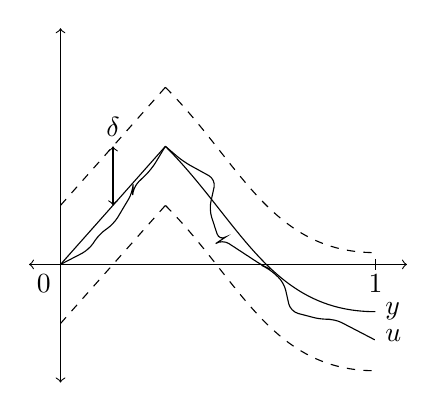
\begin{tikzpicture}[x=4cm,y=3cm,label/.style={ postaction={
          decorate,transform shape, decoration={ markings, mark=at position .8
            with \node #1;}}}]
      \pgfmathsetseed{2}
      \draw[<->] (0,1) -- (0,0)node[below left]{$0$} -- (0,-0.5);
      \draw[<->] (-0.1,0) -- (1,0)node[below]{$1$} -- (1.1,0);
      \draw[shift={(1,0)}](0pt,2pt) -- (0pt, -2pt);
      \draw (0,0) -- (0.333,0.5) (0.333,0.5) to[out=-45,in=180] (1,-0.2)node[right]{$y$};
      \draw[<->] (.1667,0.25) -- (.1667,0.50)node[above]{$\delta$};
      \draw[dashed,shift={(0,.25)}] (0,0) -- (0.333,0.5) (0.333,0.5) to[out=-45,in=180] (1,-0.2);
      \draw[dashed,shift={(0,-.25)}] (0,0) -- (0.333,0.5) (0.333,0.5) to[out=-45,in=180] (1,-0.2);
      \draw[decoration = {random steps, segment length = 3mm, amplitude = 2mm}, decorate, rounded corners=1mm]
      (0,0) -- (0.333,0.5) (0.333,0.5) to[out=-45,in=180] (1,-0.3)node[right]{$u$};
    \end{tikzpicture}
    \caption{$\hat{y}=3x+cx(1-x)\in\mathcal{V}$, $c$ arbitrary}
    \label{fig:v-equation-4}
  \end{figure}
\item $\mathcal{V} = \{y\in C^1[0,1]\;|\;y(0)=0\} \subset C^1[0,1].$
  \begin{figure}[ht]
    \centering
    \begin{subfigure}[b]{.45\textwidth}
      \centering
      \begin{tikzpicture}[yscale=.25,x=4cm,y=3cm]
        \draw[<->] (0,5) -- (0,4)node[left]{$4$} -- (0,0) -- (0,0)node[below,left]{$0$} -- (0,-2);
        \draw[->] (0,0) -- (1,0)node[below]{$1$} -- (1.1,0);
        \draw[shift={(1,0)}](0pt,2pt) -- (0pt,-2pt);
        \draw[shift={(0,4)}](2pt,0pt) -- (-2pt,0pt);
        \draw[domain=0:1,variable=\x] plot ({\x},{-(3*\x-2)^2+4});
      \end{tikzpicture}
      \caption{$y\in\mathcal{V}$}
    \end{subfigure}
    \begin{subfigure}[b]{.45\textwidth}
      \centering
      \begin{tikzpicture}[yscale=.25,x=4cm,y=3cm]
        \draw[<->] (0,5) -- (0,4)node[left]{$4$} -- (0,0) -- (0,0)node[below,left]{$0$} -- (0,-2);
        \draw[->] (0,0) -- (1,0)node[below]{$1$} -- (1.1,0);
        \draw[shift={(1,0)}](0pt,2pt) -- (0pt,-2pt);
        \draw[shift={(0,4)}](2pt,0pt) -- (-2pt,0pt);
        \draw[domain=0:1,variable=\x] plot ({\x},{-2*(3*\x-2)});
      \end{tikzpicture}
      \caption{$y'(x)$}
    \end{subfigure}
    \caption{}
    \label{fig:cn-arrrgh}
  \end{figure}
  Reference \cref{fig:cn-arrrgh}.
  \begin{equation*}
    ||y||_C^1 = \max_{0\le x\le1} |y(x)| + \max_{0\le x\le1} |y'(x)| = 4+3 = 7
  \end{equation*}
  \begin{align*}
    N_{C^1}(y,\delta)&=\{u\in\mathcal{V}\;|\;||u-y||_C^1<\delta\} \\
                     &= \left( \text{\parbox{15em}{\centering all funcs in $\mathcal{V}$ s.t.
                       $||u-y||_C^1\le\delta_0$ and $||u'-y'||_C^1\le\delta_1$ where
                       $\delta_0+\delta_1<\delta$}} \right)
  \end{align*}
\end{enumerate}
\begin{figure}[ht]
  \centering
  \begin{subfigure}[b]{.45\textwidth}
    \centering
    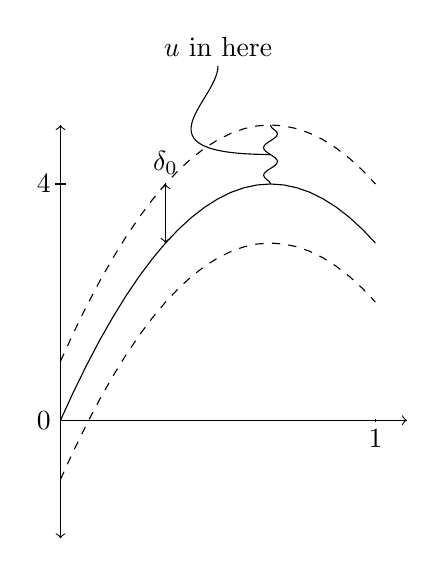
\begin{tikzpicture}[yscale=.25,x=4cm,y=3cm]
      \draw[<->] (0,5) -- (0,4)node[left]{$4$} -- (0,0) -- (0,0)node[below,left]{$0$} -- (0,-2);
      \draw[->] (0,0) -- (1,0)node[below]{$1$} -- (1.1,0);
      \draw[shift={(1,0)}](0pt,2pt) -- (0pt,-2pt);
      \draw[shift={(0,4)}](2pt,0pt) -- (-2pt,0pt);
      \draw[domain=0:1,variable=\x] plot ({\x},{-(3*\x-2)^2+4});
      \draw[shift={(0,1)},dashed,domain=0:1,variable=\x] plot ({\x},{-(3*\x-2)^2+4});
      \draw[shift={(0,-1)},dashed,domain=0:1,variable=\x] plot ({\x},{-(3*\x-2)^2+4});
      \draw[<->](.3333,2.9998) -- ++(0,1)node[above]{$\delta_0$};
      \draw[decoration=snake,decorate] (.6667,4) -- ++(0,1);
      \draw (.6667,4.5) to[out=180,in=-90] (0.5,6)node[above]{$u$ in here};
    \end{tikzpicture}
    \caption{$y\in\mathcal{V}$}
  \end{subfigure}
  \begin{subfigure}[b]{.45\textwidth}
    \centering
    \begin{tikzpicture}[yscale=.25,x=4cm,y=3cm]
      \draw[<->] (0,5) -- (0,4)node[left]{$4$} -- (0,0) -- (0,0)node[below,left]{$0$} -- (0,-2);
      \draw[->] (0,0) -- (1,0)node[below]{$1$} -- (1.1,0);
      \draw[shift={(1,0)}](0pt,2pt) -- (0pt,-2pt);
      \draw[shift={(0,4)}](2pt,0pt) -- (-2pt,0pt);
      \draw[domain=0:1,variable=\x] plot ({\x},{-2*(3*\x-2)});
      \draw[shift={(0,1)},dashed,domain=0:1,variable=\x] plot ({\x},{-2*(3*\x-2)});
      \draw[shift={(0,-1)},dashed,domain=0:.8333,variable=\x] plot ({\x},{-2*(3*\x-2)});
      \draw[<->](.3333,2.0002) -- ++(0,1)node[above]{$\delta_1$};
      \draw[decoration=snake,decorate] (.6667,0.0002) -- ++(0,1);
      \draw (.6667,0.5002) to[out=45,in=-90] (0.5,6)node[above]{$u'$ in here};
    \end{tikzpicture}
    \caption{$y'(x)$}
  \end{subfigure}
  \caption{$\delta_0+\delta_1<\delta$}
  \label{fig:cn-arrrgh2}
\end{figure}

\begin{figure}[ht]
  \centering
  \begin{tikzpicture}[yscale=.25,x=4cm,y=3cm,label/.style={ postaction={
        decorate,transform shape, decoration={ markings, mark=at position .8
          with \node #1;}}}]
    \draw[<->] (0,5) -- (0,0) -- (0,0)node[below,left]{$0$} -- (0,-2);
    \draw[->] (0,0) -- (1,0)node[below]{$1$} -- (1.1,0);
    \draw[shift={(1,0)}](0pt,2pt) -- (0pt,-2pt);
    \draw[domain=0:1,variable=\x] plot ({\x},{-(3*\x-2)^2+4}) node[right]{$y$};
    \draw[domain=0:1,variable=\x] plot ({\x},{-(3*(\x*.8)-2)^2+4})
    node[right]{$u$};
  \end{tikzpicture}
  \caption{$u\in N_{C_1}(y,\delta)$ for some $\delta\ll1$}
  \label{fig:what}
\end{figure}

\begin{figure}[ht]
  \centering
  \begin{tikzpicture}[yscale=.25,x=4cm,y=3cm,label/.style={ postaction={
        decorate,transform shape, decoration={ markings, mark=at position .8
          with \node #1;}}}]
    \draw[<->] (0,5) -- (0,0) -- (0,0)node[below,left]{$0$} -- (0,-2);
    \draw[->] (0,0) -- (1,0)node[below]{$1$} -- (1.1,0);
    \draw[shift={(1,0)}](0pt,2pt) -- (0pt,-2pt);
    \draw[domain=0:1,variable=\x] plot ({\x},{-(3*\x-2)^2+4}) node[right]{$y$};
    \draw[domain=0:.7015,variable=\x] plot ({\x},{-(3*(\x*.8)-2)^2+4.2});
    \draw[domain=.9651:1,variable=\x] plot ({\x},{-(3*(\x*.8)-2)^2+4.2})
    node[right]{$u$};
    \draw[decorate,decoration={snake, segment length=5mm, amplitude=1mm}] (.7015,4.1) -- (.9651,4.1);
  \end{tikzpicture}
  \caption{$u\cancel{\in} N_{C_1}(y,\delta)$ for some $\delta\ll1$ (because
    $u'-y'$ large at some $x$-values)}
  \label{fig:what2}
\end{figure}

See \cref{fig:cn-arrrgh2,fig:what,fig:what2}.

\subsection{Definition}
Let $\mathcal{V}\subset C^n[a,b],\; n\ge0$ and
$F:\mathcal{V}\rightarrow\mathbb{R}$ be given. An element $y_*\in\mathcal{V}$ is
called a local minimizer of $F$ in $\mathcal{V}$ in the $C^n$-norm if
$\exists\,\delta>0$ such that
$$F(u)\ge F(y_*), \quad \forall u\in N_{C^n}(y_*,\delta)$$
 or a local maximizer if
$$F(u)\le F(y_*), \quad \forall u\in N_{C^n}(y_*,\delta).$$
Local minimizers depend on how the neighborhoods are identified.

\subsection{Example}
Given
\begin{align*}
  \mathcal{V} &= \{y\in C^1[0,1] \;|\; y(0)=\alpha\} \\
  F&:\mathcal{V} \rightarrow \mathbb{R} \\
  F(y) &= \int_0^1 {(y'(x))}^2 [\beta-{(y'(x))}^2]\dd{x}
\end{align*}
where constants $\alpha, \beta > 0$.
\subsubsection*{Claim}
$F(y)$ has no absolute minimizer in $\mathbb{V}$.

Proof: Consider simple graphs $\hat{y}(x)=\alpha+cx$, where $c$ is an arbitrary
constant. Reference \cref{fig:what3}.

\begin{figure}[ht]
  \centering
  \begin{tikzpicture}[x=4cm,y=3cm,label/.style={ postaction={
        decorate,transform shape, decoration={ markings, mark=at position .8
          with \node #1;}}}]
    \draw[<->] (0,1.1) -- (0,0) -- (0,0)node[below,left]{$0$} -- (0,-.1);
    \draw[->] (0,0) -- (1,0)node[below]{$1$} -- (1.1,0);
    \draw[shift={(1,0)}](2pt,0pt) -- (-2pt,0pt);
    \draw (0,.5)node[left]{$\alpha$} -- (1,1)node[right]{$\hat{y}\in\mathcal{V}$};
    \draw (0,.5) node[circle,fill,inner sep=1pt]{};
  \end{tikzpicture}
  \caption{}
  \label{fig:what3}
\end{figure}

\begin{equation*}
  F(\hat{y}) = \int_0^1 c^2[\beta-c^2]\dd{x} = c^2(\beta-c^2)
\end{equation*}
Here, $F(\hat{y})\rightarrow -\infty$ as $|c|\rightarrow\infty$. $\therefore$ no
absolute minimum $\mathcal{V}$.

\subsubsection*{Claim}
$F(y)$ has a local minimizer in $\mathcal{V}$ in $C^1$-norm at
$y_*(x)\equiv\alpha$.

Proof:
\begin{enumerate}[(i)]
\item Reference \cref{fig:what4}.
  \begin{figure}[ht]
    \centering
    \begin{tikzpicture}[x=4cm,y=3cm,label/.style={ postaction={
          decorate,transform shape, decoration={ markings, mark=at position .8
            with \node #1;}}}]
      \draw[<->] (0,1.1) -- (0,0) -- (0,0)node[below,left]{$0$} -- (0,-.1);
      \draw[->] (0,0) -- (1,0)node[below]{$1$} -- (1.1,0);
      \draw[shift={(1,0)}](2pt,0pt) -- (-2pt,0pt);
      \draw (0,.5)node[left]{$\alpha$} -- (1,.5)node[right]{$y_*\in\mathcal{V}$};
      \draw (0,.5)node[circle,fill,inner sep=1pt]{};
    \end{tikzpicture}
    \caption{}
    \label{fig:what4}
  \end{figure}
  \begin{equation*}
    F(y_*) = \int_0^10[\beta-0]\dd{x}=0
  \end{equation*}
\item Consider $N_{C^1}(y_*,\delta)$ for any $\delta\in(0;\beta)$
  Reference \cref{fig:what5}.

\begin{figure}[ht]
  \centering
  \begin{subfigure}[b]{.45\textwidth}
    \centering
    \begin{tikzpicture}[x=4cm,y=3cm,label/.style={ postaction={
          decorate,transform shape, decoration={ markings, mark=at position .8
            with \node #1;}}}]
      \draw[<->] (0,1.1) -- (0,0) -- (0,0)node[below,left]{$0$} -- (0,-.1);
      \draw[->] (0,0) -- (1,0)node[below]{$1$} -- (1.1,0);
      \draw[shift={(1,0)}](2pt,0pt) -- (-2pt,0pt);
      \draw (0,.5)node[left]{$\alpha$} -- (1,.5)node[right]{$y_*$};
      \draw (0,.5)node[circle,fill,inner sep=1pt]{};
      \draw[dashed,shift={(0,.25)}] (0,.5) -- (1,.5);
      \draw[dashed,shift={(0,-.25)}] (0,.5) -- (1,.5);
      \draw[<->] (0.25,.5) -- (0.25,.75)node[above]{$\delta_0$};
    \end{tikzpicture}
    \caption{$y\in\mathcal{V}$}
  \end{subfigure}
  \begin{subfigure}[b]{.45\textwidth}
    \centering
    \begin{tikzpicture}[x=4cm,y=3cm,label/.style={ postaction={
          decorate,transform shape, decoration={ markings, mark=at position .8
            with \node #1;}}}]
      \draw[<->] (0,.8) -- (0,0) -- (0,0)node[below,left]{$0$} -- (0,-.4);
      \draw[->] (0,0) -- (1,0)node[below]{$1$} -- (1.1,0);
      \draw[shift={(1,0)}](2pt,0pt) -- (-2pt,0pt);
      \draw[very thick] (0,0) -- (1,0)node[above right]{$y_*'$};
      \draw[dashed,shift={(0,.25)}] (0,0) -- (1,0);
      \draw[dashed,shift={(0,-.25)}] (0,0) -- (1,0);
      \draw[<->] (.25,0) -- (.25,.25)node[above]{$\delta_1$};
    \end{tikzpicture}
    \caption{$y'(x)$}
  \end{subfigure}
  \caption{$\delta_0+\delta_1<\delta$}
  \label{fig:what5}
\end{figure}

  $$\delta_0+\delta_1<\delta$$
  For any $u\in N_{C^1}(y_*,\delta)$ we have
  \begin{align*}
    |u(x)-\alpha| &\le \delta_0 < \delta < \sqrt{\beta} \\
    |u'(x)-0| &\le \delta_1 < \delta < \sqrt{\beta} \\
  \end{align*}
  Substituting any such $u$ into $F$ gives
  \begin{equation*}
    F(u) = \int_0^1{(u'(x))}^2[\beta-{(u'(x))}^2]\dd{x} \ge 0
  \end{equation*}
  This is true for any $u$ in the neighborhood.
\item Combining (i) and (ii), we get
  \begin{equation*}
    F(u) \ge F(y_8),\quad \forall u\in N_{C^1}(y_*,\delta)
  \end{equation*}
  where $0<\delta<\sqrt{\beta}$. $\therefore y_*(x)\equiv\alpha$ is a local min
  in $C^1$-norm.
\end{enumerate}

\subsubsection*{Claim}
Although $y_*$ is a local min in $C^1$-norm, it is not a local min in
$C^0$-norm.

Proof: For any $\delta>0$ consider graphs
$$\tilde{u}(x)=\alpha+\epsilon\sin\left( \frac{x}{\epsilon^2} \right)$$
where
$$0<\epsilon<\delta,\quad 0<\epsilon\ll \beta$$
Then
\begin{enumerate}[(i)]
\item $\tilde{u}\in\mathcal{V}$
\item $\tilde{u}\in N_{C^1}(y_*,\delta)$ for any $\delta>0$
\item $F(\tilde{u})<0$ provided $0<\epsilon\ll\beta$
\end{enumerate}
$\therefore y_*$  is not a local min in $C^0$-norm.

\section{Necessary Condititions For a Local Min/Max of a Functional}
\subsection{Definition}
Consider a function space $\mathcal{V}$ of the form
\begin{equation*}
  \mathcal{V} = \{y\in C^n[a,b]\;|\;G_1(y)=c_1,\ldots,G_r(y)=c_r\}
\end{equation*}
where $G_1(y),\ldots,G_r(y)$ are given linear functionals. By the space of
admissable variations associated with $\mathcal{V}$ we mean
\begin{equation*}
  \mathcal{V} = \{y\in C^n[a,b]\;|\;G_1(y)=0,\ldots,G_r(y)=0\}
\end{equation*}
i.e. a set a conditions which satisfy a homogenous form.

\subsection{Examples}
\begin{enumerate}
\item $\mathcal{V}=\{y\in C^2[0,1]\;|\;y(0)=2,\; y'(1)=0,\; \int_0^1 y(x)\dd{x}=3\}$
  then
  \begin{equation*}
    \mathcal{V} = \{y\in C^2[0,1]\;|\;y(0)=0,\; y'(1)=0,\;\int_0^1y(x)\dd{x}=0\}.
  \end{equation*}
\item $\mathcal{V}=C^2[0,1]$ (no conditions)
  then $$\mathcal{V}_0=\mathcal{V}.$$
\end{enumerate}

\subsection{Definition}
By the variation of a graph $y_*\in\mathcal{V}$ in a direction
$h\in\mathcal{V}_0$, we mean the family of graphs
$$(y_*+\epsilon h)\in\mathcal{V},\quad \epsilon\in\mathbb{R}$$
For each $\epsilon$, $(y_*+\epsilon h)$ is a distorted version of $y_*$. The
shape of the distortion of defined by $h$.

\subsection{Example}
\begin{equation*}
  \begin{aligned}
    \mathcal{V} &= \{y\in C^2[0,1]\;|\;y(0)=0,\;y(1)=1\} \\
    \mathcal{V}_0 &= \{y\in C^2[0,1]\;|\;y(0)=0,\;y(0)=0,y(1)=0\}
  \end{aligned}
\end{equation*}
\begin{figure}[ht]
  \centering
  \begin{tikzpicture}[x=4cm,y=3cm,label/.style={ postaction={
        decorate,transform shape, decoration={ markings, mark=at position .8
          with \node #1;}}}]
    \draw[<-] (0,1.1) -- (0,1)node[left]{$1$} -- (0,0) -- (0,0)node[below,left]{$0$};
    \draw[->] (0,0) -- (1,0)node[below]{$1$} -- (1.1,0);
    \draw[shift={(0,1)}](2pt,0pt) -- (-2pt,0pt);
    \draw[shift={(1,0)}](0pt,2pt) -- (0pt,-2pt);
    \draw (0,0) -- (1,1)node[right]{$y_*\in\mathcal{V}$};
    \draw (0,0)node[circle,fill,inner sep=1pt]{};
    \draw (1,1)node[circle,fill,inner sep=1pt]{};
  \end{tikzpicture}
  \caption{}
  \label{fig:y-star-in-v}
\end{figure}
\begin{figure}[ht]
  \centering
  \begin{subfigure}[b]{.45\textwidth}
    \centering
    \begin{tikzpicture}[yscale=.5,x=4cm,y=3cm]
      \draw[<-] (0,2.1) -- (0,0) -- (0,0)node[below,left]{$0$} -- (0,-.1);
      \draw[->] (0,0) -- (1,0)node[below]{$1$} -- (1.1,0);
      \draw[shift={(1,0)}](2pt,0pt) -- (-2pt,0pt);
      \draw (1,0)node[circle,fill,inner sep=1pt]{};
      \draw (0,0)node[circle,fill,inner sep=1pt]{};
      \draw[domain=0:1,variable=\x] plot ({\x}, {sin(deg(\x*pi))});
    \end{tikzpicture}
    \caption{$h\in\mathcal{V}_0$}
  \end{subfigure}
  \begin{subfigure}[b]{.45\textwidth}
    \centering
    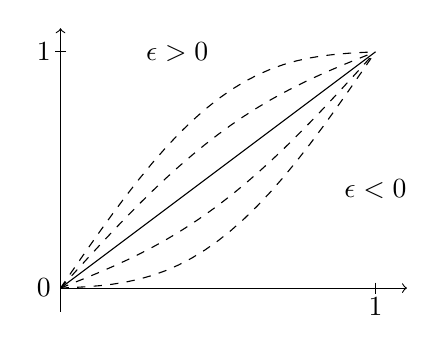
\begin{tikzpicture}[x=4cm,y=3cm]
      \draw[<-] (0,1.1) -- (0,1)node[left]{$1$} -- (0,0) -- (0,0)node[below,left]{$0$} -- (0,-.1);
      \draw[->] (0,0) -- (1,0)node[below]{$1$} -- (1.1,0);
      \draw[shift={(1,0)}](0pt,2pt) -- (0pt,-2pt);
      \draw[shift={(0,1)}](2pt,0pt) -- (-2pt,0pt);
      \pgfmathsetmacro{\eps}{.15}
      \pgfmathsetmacro{\epss}{.3}
      \draw[domain=0:1,variable=\x] plot ({\x}, {\x});
      \draw[dashed,domain=0:1,variable=\x] plot ({\x}, {\x + \eps*sin(deg(\x*pi))});
      \draw[dashed,domain=0:1,variable=\x] plot ({\x}, {\x + \epss*sin(deg(\x*pi))});
      \draw[dashed,domain=0:1,variable=\x] plot ({\x}, {\x - \eps*sin(deg(\x*pi))});
      \draw[dashed,domain=0:1,variable=\x] plot ({\x}, {\x - \epss*sin(deg(\x*pi))});
      \draw (0.5,1)node[left]{$\epsilon>0$};
      \draw (1,0.5)node[below]{$\epsilon<0$};
    \end{tikzpicture}
    \caption{$y_*+\epsilon h\in \mathcal{V}$}
  \end{subfigure}
  \caption{$h(x)=\sin x$}
  \label{fig:h-sinx}
\end{figure}
\begin{figure}[ht]
  \centering
  \begin{subfigure}[b]{.45\textwidth}
    \centering
    \begin{tikzpicture}[yscale=.25,x=4cm,y=3cm]
      \draw[<->] (0,2.1) -- (0,0) -- (0,0)node[below,left]{$0$} -- (0,-2.1);
      \draw[->] (0,0) -- (1,0)node[below]{$1$} -- (1.1,0);
      \draw[shift={(1,0)}](2pt,0pt) -- (-2pt,0pt);
      \draw (1,0)node[circle,fill,inner sep=1pt]{};
      \draw (0,0)node[circle,fill,inner sep=1pt]{};
      \draw[domain=0:1,variable=\x] plot ({\x}, {sin(deg(2*\x*pi))});
    \end{tikzpicture}
    \caption{$h\in\mathcal{V}_0$}
  \end{subfigure}
  \begin{subfigure}[b]{.45\textwidth}
    \centering
    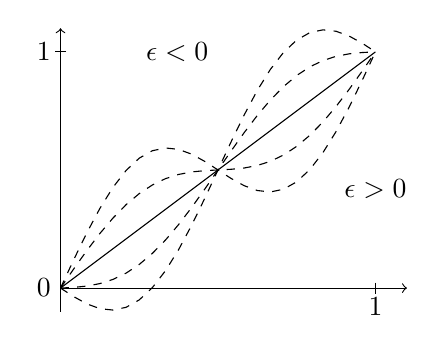
\begin{tikzpicture}[x=4cm,y=3cm]
      \draw[<-] (0,1.1) -- (0,1)node[left]{$1$} -- (0,0) -- (0,0)node[below,left]{$0$} -- (0,-.1);
      \draw[->] (0,0) -- (1,0)node[below]{$1$} -- (1.1,0);
      \draw[shift={(1,0)}](0pt,2pt) -- (0pt,-2pt);
      \draw[shift={(0,1)}](2pt,0pt) -- (-2pt,0pt);
      \pgfmathsetmacro{\eps}{.15}
      \pgfmathsetmacro{\epss}{.3}
      \draw[domain=0:1,variable=\x] plot ({\x}, {\x});
      \draw[dashed,domain=0:1,variable=\x] plot ({\x}, {\x + \eps*sin(deg(2*\x*pi))});
      \draw[dashed,domain=0:1,variable=\x] plot ({\x}, {\x + \epss*sin(deg(2*\x*pi))});
      \draw[dashed,domain=0:1,variable=\x] plot ({\x}, {\x - \eps*sin(deg(2*\x*pi))});
      \draw[dashed,domain=0:1,variable=\x] plot ({\x}, {\x - \epss*sin(deg(2*\x*pi))});
      \draw (0.5,1)node[left]{$\epsilon<0$};
      \draw (1,0.5)node[below]{$\epsilon>0$};
    \end{tikzpicture}
    \caption{$y_*+\epsilon h\in \mathcal{V}$}
  \end{subfigure}
  \caption{$h(x)=\sin(2\pi x)$}
  \label{fig:h-sinpix}
\end{figure}
Reference \cref{fig:y-star-in-v,fig:h-sinx,fig:h-sinpix}.

\subsection{Necesssary Conditions}
Let $\mathcal{V}\subset C^n[a,b],\; n\ge0$ and
$F:\mathcal{V}\rightarrow\mathbb{R}$ be given. If $y_*\in\mathcal{V}$ is a local
min of $F$ in $\mathcal{V}$ in $C^n$-norm, then we must have
\begin{equation*}
  \left[\od{}{\epsilon}F(y_*+\epsilon h)\right]_{\epsilon=0}=0,\quad \forall h\in\mathcal{V}_0
\end{equation*}
This is called the ``1st order condition''.
\begin{equation*}
  \left[\od[2]{}{\epsilon}F(y_*+\epsilon h)\right]_{\epsilon=0}\ge0,\quad \forall h\in\mathcal{V}_0
\end{equation*}
This is called the ``2nd order condition''. For a local max, change $\ge$ to $\le$.

\subsubsection{Proof}
Suppose $y_*\in\mathcal{V}$ is a local minimum of $F$. Let $h\in V_0$ be
arbitrary and define $f:\mathbb{R}\rightarrow\mathbb{R}$ by
$$f(\epsilon) = F(y_*+\epsilon h).$$
Since $y_*$ is a local minimum, we have
$$F(u)\ge F(y_*),\quad \forall u\in N_{C^n}(y_*,\delta),\;\delta>0.$$
Considering $u=y_*+\epsilon h$, this implies
$$F(y_*+\epsilon h)\ge F(y_*),\quad \forall \epsilon\in(-c,c),\; c>0.$$

\begin{figure}[ht]
  \centering
  \begin{tikzpicture}[x=4cm,y=3cm]
    \draw[<-] (0,1.1) -- (0,1)node[left]{$f$} -- (0,0) -- (0,0)node[below left]{$0$} -- (0,-.1);
    \draw[<->] (-.6,0) -- (.5,0)node[below]{$\epsilon$} -- (.6,0);
    \draw (-0.25,0)node[]{$($} (-0.25,-0.05)node[below]{$-c$};
    \draw (0.25,0)node[]{$)$} (0.25,-0.05)node[below]{$c$};
    \draw[domain=-.2165:.2165] plot ({\x}, {(\x*4)^2+.25});
  \end{tikzpicture}
  \caption{$f(\epsilon)\ge f(0)$}
  \label{fig:fepsilon-le-fzero}
\end{figure}

Reference \cref{fig:fepsilon-le-fzero}. Thus $f(\epsilon)$ has a local min at
$\epsilon=0$ and hence
\begin{equation*}
  \left[ \od{}{\epsilon}f(\epsilon) \right]_{\epsilon=0}=0,\quad
  \left[ \od[2]{}{\epsilon} f(\epsilon) \right]_{\epsilon=0}\ge0.
\end{equation*}

\subsection{Example}
\begin{equation*}
  \begin{aligned}
    \mathcal{V}&=\{y\in C^2[0,1]\;|\;y(0)=0,\; y(1)=1\} \\
    \mathcal{V}_0&= \{y\in C^2[0,1]\;|\;y(0)=0,\; y(1)=0\} \\
  \end{aligned}
\end{equation*}
$F:\mathcal{V}\rightarrow\mathbb{R}$, $F(y)=\int_0^12y(x)+{(y'(x))}^2\dd{x}$
\begin{enumerate}
\item Find an expression for
$$\left[\od{}{\epsilon}F(y+\epsilon h)\right]$$ for arbitrary $y$ and $h$
$$F(y+\epsilon h)=\int_0^1 2(y(x)+\epsilon h(x))+{(y'(x)+\epsilon h'(x))}^2\dd{x}$$
\begin{equation*}
  \begin{aligned}
    \od{}{\epsilon}F(y+\epsilon h) &=
    \od{}{\epsilon}\int_0^1 2(y(x)+\epsilon h(x))+{(y'(x)+\epsilon h'(x))}^2\dd{x} \\
    &= \int_0^1 2 h(x) + 2(y'(x)+\epsilon h'(x))h'(x)\dd{x} \\
    {\left[\od{}{\epsilon}F(y+\epsilon h)\right]}_{\epsilon=0} &= \int_0^1 2h(x)+2y'(x)h'(x)\dd{x} \\
    \delta F(y,h) &= \int_0^1 2h(x) - (2y'(x))' h(x) \dd{x} + {\left[ 2y'(x)h(x) \right]}_{x=0}^{x=1} \\
    &= \int_0^1(2-2y''(x))h(x)\dd{x} + \cancel{2h'(1)h(1)} - \cancel{2y'(0)h(0)} \\
    \implies \delta F(y,h) &= \int_0^1(2-2y'')h(x)\dd{x}.
  \end{aligned}
\end{equation*}
$\left[\od{}{\epsilon}F(y+\epsilon h)\right]_{\epsilon=0}$ is typically referred
to as $\delta F(y,h)$, read as ``1st variation of $F$ at $y$ in direction
$h$''.
\item Observe: If $y_*\in\mathcal{V}$ is a local min or max of $F$, then it must
  satisfy
$$\delta F(y_*,h)=\int_0^1(2-2y_*''(x))h(x)\dd{x}=0,\quad \forall
h\in\mathcal{V_0}$$
This condition is met when
$$2-2y_*''=0,\quad 0\le x\le 1$$
Therefore we obtain an ODE for $y_*$. This is the Euler-Lagrange equation with
boundary conditions from $\mathcal{V}$: $y_*(0)=0$ and $y_*(1)=0$. Solving gives
$$y_*(x)=\frac{1}{2}x^2 + \frac{1}{2}x.$$
\begin{figure}[ht]
  \centering
  \begin{tikzpicture}[x=4cm,y=3cm]
    \draw[<->] (0,1.1) -- (0,1)node[left]{$1$} -- (0,0) -- (0,0)node[below left]{$0$} -- (0,-.1);
    \draw[<->] (-0.1,0) -- (0,0) -- (1,0)node[below]{$1$} -- (1.1,0);
    \draw[shift={(1,0)}](0pt,2pt) -- (0pt,-2pt);
    \draw[shift={(0,1)}](2pt,0pt) -- (-2pt,0pt);
    \draw (1,1)node[circle,fill,inner sep=1pt]{};
    \draw (1,1)node[right]{$y_*\in\mathcal{V}$};
    \draw (0,0)node[circle,fill,inner sep=1pt]{};
    \draw[domain=0:1] plot ({\x}, {.5*(\x)^2+.5*\x});
  \end{tikzpicture}
  \caption{The only possible local min or max of $F$.}
  \label{fig:extremal}
\end{figure}
Reference \cref{fig:extremal}. This candidate is called the ``extremal of $F$.''
\end{enumerate}

\section{Results for 1st Order Fixed-Fixed Problems}
\subsection{Theorem}
Consider $F:\mathcal{V}\rightarrow\mathbb{R}$ of the form
$$\mathcal{V}=\{y\in C^2[a,b]\;|\;y(a)=\alpha,\;y(b)=\beta\},$$
$$F(y)=\int_a^bL(x,y,y')\dd{x}$$
where $L(x,y,y')$ is some expression in $x$, $y(x)$, and $y'(x)$.
If $y_*\in\mathcal{V}$ is a local minimizer of $F$ in the $C^2$-norm, then we
must have
\begin{equation}
  \label{eq:condition-1}
  \left[\od{}{\epsilon}F(y_*+\epsilon h)\right]_{\epsilon=0}=0\quad\forall h\in\mathcal{V}_0
\end{equation}
\begin{equation}
  \label{eq:condition-2}
  \left[\od[2]{}{\epsilon}F(y_*+\epsilon h)\right]_{\epsilon=0}\ge0  \quad\forall h\in\mathcal{V}_0
\end{equation}
The condition in \cref{eq:condition-1} implies that $y_*$ must satisfy
\begin{equation}
  \label{eq:condition-1-prime}
  (BVP)\quad\left\{
  \begin{aligned}
    \pd{L}{y}(x,y,y')-\od{}{x}\left[ \pd{L}{y'}(x,y,y') \right]=0\quad a\le x\le \\
    y(a) = \alpha,\quad y(b)=\beta
  \end{aligned} \right.
\end{equation}
The condition in \cref{eq:condition-2} implies that $y_*$ must also satisfy
\begin{equation}
  \label{eq:condition-2-prime}
  \pd[2]{L}{y'}(x,y,y')\ge0,\quad a\le x \le b
\end{equation}
For a local minimizer, change $\ge$ to $\le$ in \cref{eq:condition-2,eq:condition-2-prime}.

Sketch \cref{eq:condition-1}$\implies$\cref{eq:condition-1-prime}. Let
$y\in\mathcal{V}$, $h\in\mathcal{V}_0$ be arbitrary.
$$F(y+\epsilon h)=\int_a^bL(x,y+\epsilon h,y'+\epsilon h')\dd{x}$$
\begin{equation}
  \label{eq:something}
  \begin{aligned}
    \od{}{\epsilon}F(y+\epsilon h)&=\int_a^b\od{}{\epsilon}L(x,y+\epsilon h,y'+\epsilon h')\dd{x} \\
    &= \int_a^b\pd{L}{y}(\cdots)h + \pd{L}{y'}(\cdots)h' \dd{x} \\
    \left[\od{}{\epsilon}F(y+\epsilon h)\right]_{\epsilon=0}&=
    \int_a^b\pd{L}{y}(x,y,y')h+\pd{L}{y'}(x,y,y')h'\dd{x} \\
  \end{aligned}
\end{equation}
Let
\begin{align*}
  \delta F(y,h) &= \left[\od{}{\epsilon}F(y+\epsilon h)\right]_{\epsilon=0},\\
  g &= \pd{L}{y}(x,y,y'), \\
  f &= \pd{L}{y'}(x,y,y'). \\
\end{align*}
Then \cref{eq:something} turns to
\begin{equation*}
  \begin{aligned}
    \delta F(y,h) &= \int_a^b gh + fh' \dd{h} \\
    &= \int_a^b gh - f'h\dd{x} + \left[ fh \right]_{x=a}^{x=b} \\
    &= \int_a^b (g-f')h\dd{x}+ \cancel{\left[ fh \right]_{x=b}} - \cancel{\left[ fh \right]_{x=a}}
  \end{aligned}
\end{equation*}
The cancels occur since $h\in\mathcal{V}_0$. If $y=y_*$ is a local minimizer of
$F$, then
\begin{equation*}
  \delta F(y,h) = \int_a^b (g-f')h \dd{x}=0,\quad \forall h\in\mathcal{V}_0.
\end{equation*}
This condition can only be satisfied if $$g-f'=0,\quad a\le x \le b.$$
Substituting for $g$, $f$ gives
\begin{equation*} \left\{
  \begin{aligned}
    &\pd{L}{y}(x,y,y') - \left[ \pd{L}{y'}(x,y,y') \right]'=0,\quad a\le x \le b \\
    &y(a)=\alpha,\quad y(b)=\beta.
  \end{aligned} \right.
\end{equation*}

\subsection{Example}
$\mathcal{V}=\{y\in C^2[0,1]\;|\; y(0)=0,\; y(1)=1\}$
$$F:\mathcal{V}\rightarrow\mathbb{R}$$
$$F(y)=\int_0^12y(x)+{(y'(x))}^2\dd{x}$$
where $$L(x,y,y')=2y+{(y')}^2.$$

\begin{enumerate}
\item Find candidates for local min, max of $F$ (``extremals'').
  Derivitives of $L$:
  \begin{equation*}
    \pd{L}{y} = 2,\quad \pd{L}{y'} = 2y'
  \end{equation*}
  BVP for extremals:
  \begin{equation*} \left\{
      \begin{aligned}
        &2-\left[ 2y' \right]'=0,\quad 0\le x\le 1 \\
        &y(0)=0,\quad y(1)=1 \\
      \end{aligned} \right.
  \end{equation*}
  ODE:
  \begin{equation*}
    2-2y''=0\rightarrow y''=1, \implies y=\frac{1}{2}x^2 + (x+1)
  \end{equation*}
  BCs:
  \begin{equation*}
    \begin{aligned}
      y(0)=1&\rightarrow D=0 \\
      y(1)=1&\rightarrow \frac{1}{2}+C=1\rightarrow C=\frac{1}{2} \\
      \therefore & y_*(x) = \frac{1}{2}x^2 + \frac{1}{2} x
    \end{aligned}
  \end{equation*}
  Here, $y_*$ is the only candidate for a local min/max.
\item Use the condition in \cref{eq:condition-2-prime} to further classify
  candidates. Derivitives of $L$:
  \begin{equation*}
    \pd{L}{y'}=2y',\quad \pd[2]{L}{y'}=2
  \end{equation*}
  Sign condition
  \begin{equation*}
    \pd[2]{L}{y'}(x,y_*,y_*')\equiv 2\ge0,\quad 0\le x \le1.
  \end{equation*}
  $\therefore$ $y_*$ could be a local min but not a local max.
\item Is $y_*$ actually a local minimizer of $F$? Yes.
  \subsubsection{Proof}
  Consider $\delta>0$ be given. Consider any $u\in N_{C^2}(y_*,\delta)$ and let
  $h=u-y_*$. Then $h\in\mathcal{V}_0$ and

  \begin{equation*}
    \begin{aligned}
      F(u)&=F(y_*+h) \\
      &= \int_a^b 2(y_*+h)+{(y_*'+h')}^2\dd{x} \\
      &= \int_a^b 2y_* + {(y_*')}^2\dd{x} + \int_a^b 2h\dd{x} + \int_a^b 2y_*'h'\dd{x} + \int {(h')}^2\dd{x} \\
      &= F(y_*) + \int_0^1 2h + 2y_*'h'\dd{x} + \int_0^1{(h')}^2\dd{x} \\
      &= F(y_*) + \cancel{\int_0^1(2-2y_*'')h\dd{x}} + \int_0^1{(h')}^2\dd{x} \\
      \therefore F(u) - F(y_*) &= \int_0^1{(h')}^2\dd{x} \ge 0 \\
      \therefore F(u) &\ge F(y_*) \quad \forall u\in N_{C^2}(y_*,\delta)
    \end{aligned}
  \end{equation*}
  $\therefore$ $y_*$ is a local min of $F$ (actually absolute min since no
  conditions on $\delta>0$).
\end{enumerate}

\section{Case Study: Design of a Slide}
\subsection{Problem}
Consider desigining a slide of given height $h$, length $\ell$, initial speed
$c$, and gravity $g$. See pic. 1. We seek a profile which minimizes the travel
time $T$ down the slide.

\subsubsection{Travel Time}
Since $T$ depends on the profile curve, we have
$$T=F(y),$$ where $F(y)$ is some functional. To find $F$, consider a mass $m$
sliding down profile $y(x)$. Compute the time to travel across cross a given
profile. See pic. 2. Let
\begin{align*}
  (x(t),y(x(t))) &= \text{position}\;t\ge0 \\
  \left(\od{x}{t},\od{y}{t}\right) &= (u,v) = \text{velocity}\;t\ge0
\end{align*}
Notice
$$v=\od{y}{t}=\od{y}{x}\od{x}{t}=\od{y}{x}u.$$
Assuming no friction or air resistance, conservation of energy requires
\begin{equation*}
  \left( \text{\parbox{7em}{\centering total energy at time $t\ge0$}} \right) =
  \left( \text{\parbox{7em}{\centering total energy at time $t=0$}} \right)
\end{equation*}
Therefore
\begin{equation}
  \label{eq:energy-equation}
  \frac{1}{2}m(u^2+v^2)+mgy = \frac{1}{2}m(u_0^2+v_0^2)+mgy_0
\end{equation}
Let $v^2={\left( \od{y}{x} \right)}^2u^2$, $c^2=u_0^2+v_0^2$, and $h=y_0$, where
$c^2$ and $h$ are given constants. Multiplying \cref{eq:energy-equation} by
$2/m$ gives
\begin{equation*}
  u^2\left[ 1+{\left( \od{y}{x} \right)}^2 \right]+2gy = c^2+2gh
\end{equation*}
so that
\begin{equation*}
  u^2 = \frac{c^2+2gh(h-y)}{1+{\left( \od{y}{x} \right)}^2}
\end{equation*}
Assuming $u=\od{x}{t}\ge0$ throughout the travel, we get
\begin{equation*}
  \od{x}{t} = {\left[ \frac{c^2+2g(h-y)}{1+{(y')}^2} \right]}^{1/2}
\end{equation*}
The travel time $T$ for a profile $y(x)$ is
\begin{equation*}
  T=\int_{t=0}^{t=T} \dd{t}.
\end{equation*}
Through a change of variable we obtain
\begin{equation*}
  T=\int_{x=0}^{x=\ell} \od{t}{x} \dd{x}
  = \int_0^{\ell} {\left[ \frac{1+{(y'(x))}^2}{c^2+2gh(h-y(x))} \right]}^{1/2} \dd{x}.
\end{equation*}

\subsection{Restated Problem}
Consider $F:\mathcal{V}\rightarrow\mathbb{R}$ where
\begin{equation*}
  F(y)=\int_0^{\ell}  {\left[ \frac{1+{(y'(x))}^2}{c^2+2gh(h-y(x))} \right]}^{1/2} \dd{x}.
\end{equation*}
Let $L(x,y,y')= {\left[ \frac{1+{(y'(x))}^2}{c^2+2g(h-y(x))} \right]}^{1/2} \dd{x}$.

Consider $\mathcal{V}=\{y\in C^2[0,1]\;|\;y(0)=h,\; y(\ell)=0\;,
y(x)<(h+c^2/2g)\}.$ See pic. 3. We seek local minimizers of $F$ in
$\mathcal{V}$.

\subsubsection{Necessary Condition}
Every candidate for a local minimum must satisfy

\begin{align*}
  \text{(ODE)}
  &\qquad \pd{L}{y}(x,y,y')-\od{}{x}\left[ \pd{L}{y'}(x,y,y') \right]=0,\quad 0\le x\le \ell\\
  \text{(BCs)}
  &\qquad y(0)=h,\quad h(\ell)=0.
\end{align*}
This becomes very difficult, though we may simpilfy.

\subsubsection{Simplification of ODE}
ODE can be simplified when $L(x,y,y')$ is independent of $x$.
\begin{equation*}
  L(x,y,y')=\frac{{[1+{(y')}^2]}^{1/2}}{{[c^2+2g(h-y)]}^{1/2}} = M(y,y')
\end{equation*}

\begin{equation}
  \label{eq:m-equation}
  \text{(ODE)}\quad\longleftrightarrow \quad 0=\pd{M}{y}- \od{}{x}\left[ \pd{M}{y'} \right]
\end{equation}
Multiplying \cref{eq:m-equation} by $y'$, using the derivative
formula\footnote{$f'y'=(fy')'-fy''$} and then applying the chain rule:
\begin{align*}
  0 &= \pd{M}{y} y' - \od{}{x}\left[ \pd{M}{y'} \right]y' \\
    &= \pd{M}{y}y' + \left[ \pd{M}{y'} \right]y'' - \od{}{x}\left[ \pd{M}{y'}y' \right] \\
    &= \od{}{x}\left[ M(y,y') \right] - \od{}{x}\left[ \pd{M}{y'}y' \right]
\end{align*}
This allows us to integrate once
\begin{equation*}
  A = M(y,y')-\pd{M}{y'}(y,y')y',
\end{equation*}
where $A$ is an arbitrary constant. Substituting for $M$, the ODE becomes
\begin{align*}
  A
  &= \frac{{\left[ 1+{(y')}^2 \right]}^{1/2}}{{\left[ c^2+2g(h-y) \right]}^{1/2}} -
    \frac{\frac{1}{2}{\left[ 1+{(y')}^2 \right]}^{-1/2}2y'}{{\left[ c^2+2g(h-y) \right]}^{1/2}}y' \\
  A{{\left[ c^2+2g(h-y) \right]}^{1/2}}
  &= {\left[ 1+{(y')}^2 \right]}^{1/2} -
    {\left[ 1+{(y')}^2 \right]}^{-1/2}{(y')}^2 \\
  &= {\left[ 1+ {(y')}^2 \right]}^{-1/2} \\
  A^2{\left[ c^2+2g(h-y) \right]}
  &= {\left[ 1+ {(y')}^2 \right]}^{-1} \\
\end{align*}
Let
\begin{align*}
  \gamma &= c^2+2gh > 0 \\
  \eta &= 2g
\end{align*}
\begin{align*}
  1 + {(y')}^2 &= \frac{1}{a^2[\gamma-\eta y]} \\
  {(y')}^2 &= \frac{1}{A[\gamma-\eta y]}-1 \\
  \implies {(y')}^2 &= \frac{1-A^2[\gamma-\eta y]}{A^2[\gamma-\eta y]} \\
\end{align*}
Hence every candidate for a local minimum must satisfy
\begin{align*}
  {\left( \od{y}{x} \right)}^2 &= \frac{B-(\gamma-\eta y)}{(\gamma-\eta y)},\quad 0\le x \le \ell \\
  y(0)&=h, \quad y(\ell)=0
\end{align*}
where $B>0$ is an arbitrary constant.

\end{document}
